%\algnewcommand{\IfNDebug}[1]{#1}
%\algnewcommand{\IfNDebug}[1]{}

\newcommand{\varStartG}{\ensuremath{\AlgVar{start}_G}}
\newcommand{\varEndG}{\ensuremath{\AlgVar{end}_G}}
\newcommand{\varStartH}{\ensuremath{\AlgVar{start}_H}}
\newcommand{\varEndH}{\ensuremath{\AlgVar{end}_H}}
\newcommand{\varActive}{\ensuremath{\AlgVar{active}}}
\newcommand{\varSplitting}{\ensuremath{\AlgVar{splitting}}}
\newcommand{\varPrev}{\ensuremath{\AlgVar{prev}}}
\newcommand{\varNext}{\ensuremath{\AlgVar{next}}}
\newcommand{\labelClass}{\ensuremath{\AlgVar{labelClass}}}
\newcommand{\vertexPtr}{\ensuremath{\AlgVar{vertexPtr}}}
\newcommand{\calLC}{\ensuremath{\mathcal{LC}}}
\newcommand{\LC}{\ensuremath{\AlgVar{LC}}}
\newcommand{\Gptrs}{\ensuremath{\AlgVar{Gptrs}}}
\newcommand{\Hptrs}{\ensuremath{\AlgVar{Hptrs}}}
\newcommand{\Garray}{\ensuremath{A_G}}
\newcommand{\Harray}{\ensuremath{A_H}}

\chapter{McSplit-SI: An algorithm for the induced subgraph isomorphism problem}
\label{c:mcsplit-si}

\section{Introduction}

In the induced subgraph isomorphism problem, we seek an induced copy of pattern graph $G$ in target graph $H$. This is a special case of the decision version of maximum common induced subgraph in which we require the common subgraph to contain all of graph $G$'s vertices.

The \McSplit\ algorithm may be trivially modified to solve the induced subgraph isomorphism problem. Rather than calculating an upper bound at each search node, we simply backtrack when the $G$-set of any label class is larger than the corresponding $H$-set, since by the pigeonhole principle this implies that we cannot map each pattern-graph vertex to a target-graph vertex.

While \McSplit\ is well suited to the small (tens of vertices), relatively dense pattern and target graphs that are typical of maximum common subgraph instances, it has two disadvantages for large (hundreds or thousands of vertices), sparse graphs that appear in benchmark instances for subgraph isomorphism.  The first disadvantage relates to space: $b(n_G^2 + n_H^2)$ space is needed to store the adjacency matrices, where $b$ is the memory size of a boolean variable.\footnote{We could switch to a more space-efficient representation such as hash-sets of neighbours which would still permit amortized constant time adjacency tests in the algorithm's partitioning step, but this would slow down the algorithm significantly.}  The second disadvantage relates to time: during the partitioning step, the \McSplit\ algorithm iterates over all of the vertices in each label class, which often requires checking close to $n_G + n_H$ adjacency-matrix elements each time the partitioning procedure is carried out.

\begin{figure}[htb]
    \centering
    \includegraphics*[width=0.6\textwidth]{14b-mcsplit-induced-si/density-chart/plots/n-density-pdf}
    \caption{Number of vertices and density (log scale) for each target graph in the benchmark set
    of $14,621$ subgraph isomorphism decision instances.}
    \label{figure:si-targets-n-density}
\end{figure}

\Cref{figure:si-targets-n-density} shows vertex count and density for the target graphs of the benchmark instances
that we will use in this chapter.  Of the entire benchmark set, $76\%$ of pattern graphs have density less than $0.01$.  Thus, it would
greatly improve our \McSplit\ algorithm for subgraph isomorphism on these and similar instances if we could reduce the time complexity of the partitioning
step from $O(n_G + n_H)$ to $O(|N(v)| + |N(w)|)$, where $(v,w)$ is the most-recently made mapping of a pattern vertex to a target
vertex.  In this chapter we introduce this improved algorithm, which we call \McSplit-SI.

\FloatBarrier

\section{The label class object}

In the basic version of the \McSplit\ algorithm that was described in
\Cref{c:mcsplit-i-undirected}, the label class objects at each level of the search tree are stored
contiguously in an array, and each object representing
a label class $\langle S_G, S_H \rangle$ requires only four indices or pointers: to the start and
end of the array slices that contain $S_G$ and $S_H$.
To enable partitioning in $O(|N_G(v)| + |N_H(w)|)$ time, \McSplit-SI
requires a more elaborate label-class object, and stores the objects in a doubly-linked list which is modified
when partitioning domains and restored on backtracking.

\Cref{tab:mcsplit-si-object} lists the member variables of a label class object.
The first two members are $\AlgVar{prev}$ and $\AlgVar{next}$ pointers, which
allow the set of label classes to be jointed together as a doubly-linked list.
These pointers are useful not only for iterating over the list but also
for restoring deleted elements when backtracking, as we will discuss later in the chapter.

The next four members of the object play the same role as the four indices used in \McSplit's
simpler label class object: they point to the ranges in the permuations of $V(G)$ and $V(H)$ that
contain $S_G$ and $S_H$.

Finally, we have two boolean flags, $\varActive$ and $\varSplitting$.  The first flag
records whether the label class object is currently in the list of label classes.  (Inactive
label classes have been deleted, but are maintained in memory so that they can be restored
when backtracking.)  The second flag is used temporarily during the partitioning step
to record which label class have been partitioned.

\begin{table}[htb]
\centering
\footnotesize
 \begin{tabular}{p{0.13\linewidth} p{0.2\linewidth} p{0.5\linewidth}}
 \toprule
    Name & Type & Description \\ [0.5ex]
 \midrule
    $\AlgVar{prev}$ & Pointer to Label Class & The previous label class in the doubly-linked list of all label classes \\
    \rule{0pt}{2.3ex}$\AlgVar{next}$ & Pointer to Label Class & The next label class in the doubly-linked list of all label classes \\
    \rule{0pt}{2.3ex}\varStartG & Pointer to Integer & Pointer to the first vertex of the $G$-set\\
    \rule{0pt}{2.3ex}\varEndG & Pointer to Integer & Pointer to one element past the last vertex of the $G$-set\\
    \rule{0pt}{2.3ex}\varStartH & Pointer to Integer & Pointer to the first vertex of the $H$-set\\
    \rule{0pt}{2.3ex}\varEndH & Pointer to Integer & Pointer to one element past the last vertex of the $H$-set\\
    \rule{0pt}{2.3ex}$\AlgVar{active}$ & Boolean & Is this label class in the doubly linked list? \\
    \rule{0pt}{2.3ex}$\AlgVar{splitting}$ & Boolean & Is this label class being split? \\
 \bottomrule
\end{tabular}
\caption{The member variables of \McSplit-SI label class object}
\label{tab:mcsplit-si-object}
\end{table}

The collection of data structures used by \McSplit-SI to represent the set of active label
classes has three components.  The first of these is the the doubly-linked list of label
class objects that we have described; we refer to this as \calLC.  The second 
component is the pair of arrays that store partitions of $V(G)$ and $V(H)$ that are pointed
to by each label class object.   We call these arrays $\Garray$ and $\Harray$.

The final component of our collection of data structures contains two arrays, $\Gptrs$
and $\Hptrs$.  These contain
an object for each vertex $v$ of $G$ and $H$ respectively.  Each object contains two pointers.
The first pointer of $\Gptrs[v]$ points to the position in $\Garray$ at which $v$
appears, and the second points to the label class containing $v$.
Similarly, the pointers of $\Hptrs[w]$ point to the position in $\Harray$ at which $w$
appears and the label class containing $w$.
The arrays $\AlgVar{Gptrs}$ and $\AlgVar{Hptrs}$ allows us to perform constant-time
manipulations to label classes given only a vertex; it is these arrays that enable
\McSplit-SI to carry out the partitioning step without iterating over the vertices in each label class.

TODO move this sentence:
Initially, the doubly-linked list of label classes contains a single element representing
all vertices of graphs $G$ and $H$.

\begin{figure}[h!]
    \centering
    \scalebox{.8}{
        \tikz {
            \graph [nodes={draw, circle, minimum width=.55cm, inner sep=1pt}, circular placement, radius=0.95cm,
                    clockwise=5] {
                        1,2,3,4,5;
                1--4; 1--5; 2--3; 2--5; 3--5;
            };
        }
        \qquad\qquad
        \tikz {
            \graph [nodes={draw, circle, minimum width=.55cm, inner sep=1pt}, circular placement, radius=0.95cm,
                    clockwise=6, phase=60] {
                        a,b,c,d,e,f;
                a--b; a--c; a--e; b--d; b--f; c--d; c--e; c--f; d--f; e--f;
            };
        }
    }
    \caption{Example graphs $G$ and $H$}
    \label{figure:example-g-and-h-redux}
\end{figure}

\Cref{figure:example-g-and-h-redux} reproduces, for convenience, the example
graphs from \Cref{c:mcsplit-i-undirected} which we will also use for our running example
in this chapter.
\Cref{figure:si-data-structures} shows the data structures of \McSplit-SI
after making the assignment $(1,a)$ in the induced subgraph isomorphism instance with pattern
graph $G$ and target graph $H$.  In the middle row of the figure we have the doubly-linked
list $\calLC$.  Immediately above and below this are the $\Garray$ and $\Harray$ arrays.
At the top and bottom are the arrays $\Gptrs$ and $\Hptrs$.

\begin{figure}[htb]
    \centering
    \includegraphics*[width=0.9\textwidth]{14b-mcsplit-induced-si/figs/data-structure-step-1}
    \caption{The data structures of \McSplit-SI after assigning vertex $1$ to vertex $a$.
        Circles represent pointers; hollow circles are null pointers.  The middle row shows
        the doubly-linked list of label classes.  Shown immediately above and below this are the
        permutations of $V(G)$ and $V(H)$, stored as arrays.  The top and bottom rows
        show the arrays $\AlgVar{Gptrs}$ and $\AlgVar{Hptrs}$.  Each element of these arrays
        corresponds to a vertex $v$ of $G$ or $H$, and points to the position of $v$
        the permutation and to the label class containing $v$.  To reduce clutter in the diagram,
        the label class pointers are shown pointing to a rectangle of the same colour as the
        label class.}
    \label{figure:si-data-structures}
\end{figure}

\FloatBarrier

\section{The algorithm}

\Cref{McSplitSIAlg} presents the overall structure of \McSplit-SI.  The entry point is
on \lineref{McSplitSIFun}.  If $G$ has more vertices than $H$, the instance is trivially
unsatisfiable. Otherwise, the global data label-class data structures are set up with
a single label class, and the main recursive function $\FuncSty{Search}$ is called with
an empty mapping.

\Lineref{McSplitSIReturnTrue} returns true if a mapping containing all vertices of the
pattern graph has been found.  Otherwise, the algorithm selects a label class
$\langle S_G, S_H \rangle$, and from within $S_G$ a vertex on which to branch.
(We will discuss variable selection heuristics in section ...) We then iterate
over the vertices $w$ in $S_H$, attemptying to map $v$ to $w$.

\begin{algorithm}[htb]
\AlgorithmFontSize
\DontPrintSemicolon
\nl $\FuncSty{Search}(M)$ \;
\nl \Begin{
    \nl \lIf {$|M| = |V(G)|$}{\KwSty{return} $\AlgVar{true}$} \label{McSplitSIReturnTrue}
\medskip
\nl $\langle \setG,\setH \rangle \gets \FuncSty{SelectLabelClass}()$ \label{McSplitSISelectClass} \;
\nl $v \gets \FuncSty{SelectVertex}(\setG)$ \label{McSplitSISelectVertex} \;
    \nl \For {$w \in \setH$ \label{McSplitSIWLoop}} {
\nl    $\FuncSty{Assign}(v,w)$ \;
\nl    $(\AlgVar{splits}, \AlgVar{deletions}, \AlgVar{failed}) \gets \FuncSty{Filter}(v, w)$ \;
\nl    \If{$\AlgVar{failed}$}{
\nl        $\AlgVar{success} \gets \AlgVar{false}$ \;
       }
\nl    \Else {
\nl        $\AlgVar{success} \gets \FuncSty{Search}(M \cup \{(v,w)\})$ \;
\nl        $\FuncSty{Unfilter}(\AlgVar{splits}, \AlgVar{deletions})$ \;
       }
\nl    $\FuncSty{Unassign}(v,w,\langle \setG,\setH \rangle)$ \;
\nl    \lIf {$\AlgVar{success}$}{$\KwSty{return}$ $\AlgVar{true}$}
  }
\nl  $\KwSty{return}$ $\AlgVar{false}$\;
}
\;
\nl $\FuncSty{McSplitSI}(\graphG,\graphH)$ \label{McSplitSIFun} \;
\nl \Begin{
\nl \lIf {$|V(G)| > |V(H)|$}{\KwSty{return} $\AlgVar{false}$}
\nl Initialise global data structure with the label class $\{\langle V(\graphG),V(\graphH) \rangle \}$ \;
\nl $\KwSty{return}$ $\FuncSty{Search}(\emptyset)$ \label{McSplitSIFirstExpandCall} \;
}
\caption{\McSplit-SI}
\label{McSplitSIAlg}
\end{algorithm}

Within this loop, we have two pairs of functions:
$\FuncSty{Assign}$ / $\FuncSty{Unassign}$
and
$\FuncSty{Filter}$ / $\FuncSty{Unfilter}$.  In each pair, the
second function reverses the action of the first on the global
data structure of label classes.

The first pair of functions is shown in \Cref{McSplitSIAlgAssign}.
Both of these run in constant time.
The function $\FuncSty{Assign}(v,w)$ updates the label classes to reflect
the assignment of $v$ in the pattern graph to $w$ in the target graph.  It 
does this by moving $v$ and $w$ to the end of their label class in
$\Garray$ and $\Harray$, then decrementing the end pointers of the label class.
If no vertices of the pattern graph remain in the label class, the label-class
object is deleted from the linked list $\calLC$.

In addition, to maintain the invariants of
the $\AlgVar{Gptrs}$ and $\AlgVar{Hptrs}$ arrays, we set the label-class pointers of
$\AlgVar{Gptrs}[v]$ and $\AlgVar{Hptrs}[w]$ to null since these vertices
are no longer in a label class, and update the vertex pointers
for $v$, $w$, and the vertices with which these were swapped to point to these
vertices' new positions in the $V_G$ and $V_H$ arrays.
\Cref{figure:si-data-structures-2} shows the data structures after the assignment
of $2$ to $d$ in our example.

\begin{algorithm}[htb]
\AlgorithmFontSize
\DontPrintSemicolon
\nl $\FuncSty{Assign}(v,w)$ \;
\nl \Begin{
\nl   $\LC \gets \Gptrs[v].\labelClass$ \;
\medskip
\nl   \LeftComment{delete $v$ from \LC} \;
\nl   $u \gets$ the vertex in $\Garray$ whose address is one element before $\LC.\AlgVar{end}_G$ \;
\nl   Swap $v$ with $u$ in $\Garray$, using the address of $v$ in $\Gptrs[v].\vertexPtr$ \;
\nl   Swap $\Gptrs[v].\vertexPtr$ with $\Gptrs[u].\vertexPtr$ \;
\nl   Decrement $\LC.\AlgVar{end}_G$ \;
\nl   $\Gptrs[v].\labelClass \gets \AlgVar{null}$ \;
\medskip
\nl   \LeftComment{delete $w$ from \LC} \;
\nl   $u \gets$ the vertex in $\Harray$ whose address is one element before $\LC.\AlgVar{end}_H$ \;
\nl   Swap $w$ with $u$ in $\Harray$, using the address of $w$ in $\Hptrs[w].\vertexPtr$ \;
\nl   Swap $\Hptrs[w].\vertexPtr$ with $\Hptrs[u].\vertexPtr$ \;
\nl   Decrement $\LC.\AlgVar{end}_H$ \;
\nl   $\Hptrs[w].\labelClass \gets \AlgVar{null}$ \;
\medskip
\nl   \If{$\LC.\varStartG = \LC.\varEndG$}{
\nl     \LeftComment{Delete $\LC$ from the doubly linked list of label classes} \;
\nl     $\LC.\varPrev.\varNext \gets \LC.\varNext$ \;
\nl     $\LC.\varNext.\varPrev \gets \LC.\varPrev$ \;
      }
}
\;
\nl $\FuncSty{Unassign}(v,w,\LC)$ \;
\nl \Begin{
\nl   \If{$\LC.\varStartG = \LC.\varEndG$}{
\nl     \LeftComment{Restore $\LC$ to the doubly linked list of label classes} \;
\nl     $\LC.\varPrev.\varNext \gets \LC$ \;
\nl     $\LC.\varNext.\varPrev \gets \LC$ \;
      }
\medskip
\nl   \LeftComment{restore $v$ and $w$ to \LC} \;
\nl   $\Gptrs[v].\labelClass \gets \LC$ \;
\nl   $\Hptrs[w].\labelClass \gets \LC$ \;
\nl   Increment $\LC.\AlgVar{end}_G$ \;
\nl   Increment $\LC.\AlgVar{end}_H$ \;
}
\caption{The $\FuncSty{Assign}$ and $\FuncSty{Unassign}$ functions of \McSplit-SI}
\label{McSplitSIAlgAssign}
\end{algorithm}

\begin{figure}[htb]
    \centering
    \includegraphics*[width=0.9\textwidth]{14b-mcsplit-induced-si/figs/data-structure-step-2}
    \caption{The data structures after mapping vertex $2$ to vertex $d$.}
    \label{figure:si-data-structures-2}
\end{figure}

\FloatBarrier

\section{The partitioning algorithm}

We now describe the partitioning step, referring in our running example to
the refinement of label classes carried out after mapping $2$ to $d$.
\Cref{figure:si-data-structures-3} shows the data structures after this step is completed.

\begin{figure}[htb]
    \centering
    \includegraphics*[width=0.9\textwidth]{14b-mcsplit-induced-si/figs/data-structure-step-3}
    \caption{The data structures after partitioning}
    \label{figure:si-data-structures-3}
\end{figure}

Each label class object that contained the sets $\langle V_G, V_H \rangle$ prior
to the partitioning process contains $\langle V_G \setminus N_G(v), V_H \setminus N_H(w)\rangle$
at the end of the partitioning process.  If either $V_G \cap H_G(v)$ or $V_H \cap N_H(w)$
is non-empty, the partitioning process creates a new label class object
$\langle V_G \cap N_G(v), V_H \cap N_H(w)\rangle$ which is
positioned in the doubly linked list immediately after the original label class.
To carry out the process, we iterate over $N_G(v)$ then $N_H(w)$,
creating new label classes as required, as shown in the function $\FuncSty{Filter}$
in \Cref{McSplitSIAlgFilter}.

\begin{algorithm}[htb]
\AlgorithmFontSize
\DontPrintSemicolon
\nl $\FuncSty{Filter}(v,w)$ \;
\nl \Begin{
\nl  $\AlgVar{splits} \gets []$  \LeftComment{Initialise array of pointers to split label classes} \;
\medskip 
\nl  \LeftComment{For each neighbour of $v$ that is is a label class, move $v$ into a new label class} \;
\nl  \For {$u \in \N_G(v)$\label{FilterGLoop}} {
\nl      $\LC \gets \Gptrs[u].\labelClass$ \;
\nl      \If{$\LC = \AlgVar{null}$}{
\nl          \LeftComment{$u$ is already in $M$, and therefore not in any label class} \;
\nl          \KwSty{continue} \;
         }
\nl      \If{$\LC.\varSplitting = \AlgVar{false}$}{
\nl          $\LC.\varSplitting \gets \AlgVar{true}$ \;
\nl          $\FuncSty{CreateLabelClassAfter}(\LC)$ \;
\nl          Append to $\AlgVar{splits}$ a pointer to \LC \;
         }
\nl      Swap $u$ to the end of $\LC$ in \Garray, updating the relevant $\vertexPtr$ members in \Gptrs \;
\nl      Decrement $\LC.\varEndG$  \LeftComment{Delete $u$ from $\LC$} \;
\nl      Decrement $\LC'.\varStartG$  \LeftComment{Add $u$ to $\LC'$} \;
    }
\medskip 
\nl  \LeftComment{For each neighbour of $w$ that is is a label class, move $w$ into a new label class} \;
\nl  \For {$u \in \N_H(w)$\label{FilterHLoop}} {
\nl      $\LC \gets \Hptrs[u].\labelClass$ \;
\nl      \If{$\LC = \AlgVar{null}$}{
\nl          \LeftComment{$u$ is already in $M$, and therefore not in any label class} \;
\nl          \KwSty{continue} \;
         }
\nl      \If{$\LC.\varActive = \AlgVar{false}$}{
\nl          \LeftComment{The label class containing $u$ was deleted at a shallower level of the search tree} \;
\nl          \KwSty{continue} \;
         }
\nl      \If{$\LC.\varSplitting = \AlgVar{false}$}{
\nl          $\LC.\varSplitting \gets \AlgVar{true}$ \;
\nl          $\FuncSty{CreateLabelClassAfter}(\LC)$ \;
\nl          Append to $\AlgVar{splits}$ a pointer to \LC \;
         }
\nl      Swap $u$ to the end of $\LC$ in \Harray, updating the relevant $\vertexPtr$ members in \Hptrs \;
\nl      Decrement $\LC.\varEndH$  \LeftComment{Delete $u$ from $\LC$} \;
\nl      Decrement $\LC'.\varStartH$  \LeftComment{Add $u$ to $\LC'$} \;
    }
\medskip
\nl  \For {$\LC \in \AlgVar{splits}$} {
\nl     $\LC.\varSplitting \gets \AlgVar{false}$ \;
}
\medskip
\nl  \For {$\LC \in \AlgVar{splits}$} {
\nl     \If{$\LC.\varEndG - \LC.\varStartG > \LC.\varEndH - \LC.\varStartH$}{
\nl         $\KwSty{return}$ $([],[],\AlgVar{true})$
}
\nl     \If{$\LC.next.\varEndG - \LC.next.\varStartG > \LC.next.\varEndH - \LC.next.\varStartH$}{
\nl         $\KwSty{return}$ $([],[],\AlgVar{true})$
}
}
\medskip
\nl  $\AlgVar{deletions} \gets \FuncSty{DoDeletions}(\AlgVar{splits})$ \label{McSplitSIDoDeletions}\;
\medskip
\nl  $\KwSty{return}$ $(\AlgVar{splits}, \AlgVar{deletions}, \AlgVar{false})$ \label{ReturnFromFilter}\;
}
\;
\nl $\FuncSty{CreateLabelClassAfter}(\LC)$ \;
\nl \Begin{
\nl    Insert a new label class object $\LC'$ after $\LC$ in the doubly linked list \;
\nl    $\LC'.\varStartG \gets \LC.\varEndG$ \;
\nl    $\LC'.\varEndG \gets \LC.\varEndG$ \;
\nl    $\LC'.\varStartH \gets \LC.\varEndH$ \;
\nl    $\LC'.\varEndH \gets \LC.\varEndH$ \;
\nl    $\LC'.\varActive \gets \AlgVar{true}$ \;
\nl    $\LC'.\varSplitting \gets \AlgVar{false}$ \;
}
\caption{The $\FuncSty{Filter}$ function}
\label{McSplitSIAlgFilter}
\end{algorithm}

\FloatBarrier

\section{Cleanup}

In \Cref{figure:si-data-structures-3}, we can see that the first label class
now contains no elements of $V_G$.  As a result, we can safely delete this label
class object from the linked list.  The general procedure of deletion is as
follows.\footnote{Our implementation has an extra pointer within each label
class object so we can store the deleted\_label\_classes list as a linked list
without the need for an external array of pointers.}


\begin{algorithm}[htb]
\AlgorithmFontSize
\DontPrintSemicolon
\nl $\FuncSty{DoDeletions}(\AlgVar{splits})$ \;
\nl \Begin{
\nl   $\AlgVar{deletions} \gets []$  \LeftComment{Initialise list of pointers to deleted label classes} \;
\medskip 
\nl   \For {$\LC \in \AlgVar{splits}$} {
\nl     \If {$\LC.\varStartG = \LC.\varEndG$} {
            $\FuncSty{DeleteLabelClass}(\LC)$
            Append $\LC$ to $\AlgVar{deletions}$
        } 
\nl     \If {$\LC.next.\varStartG = \LC.next.\varEndG$} {
            $\FuncSty{DeleteLabelClass}(\LC.next)$
            Append $\LC.next$ to $\AlgVar{deletions}$
        } 
    }
    $\KwSty{return}$ $\AlgVar{deletions}$ \;
}
\;
\nl $\FuncSty{DeleteLabelClass}(\LC)$ \;
\nl \Begin{
\nl     $\LC.\varPrev.\varNext \gets \AlgVar{null}$ \;
\nl     $\LC.\varNext.\varPrev \gets \AlgVar{null}$ \;
\nl     $\LC.\varActive \gets \AlgVar{false}$
}
\caption{The $\FuncSty{DoDeletions}$ function}
\label{McSplitSIAlgDelete}
\end{algorithm}

We do not garbage-collect this label class, and
we leave its $\AlgVar{prev}$ and $\AlgVar{next}$ 
pointers unchanged; we will use these pointers' values to return
the label class to the doubly linked list when backtracking.

After calling the $\FuncSty{DoDeletions}$ function,
the $\FuncSty{Filter}$ function returns on \lineref{ReturnFromFilter} 
of \Cref{McSplitSIAlgFilter}.  Three values are returned. The lists
of split label classes and deleted label classes will be used to restore
the data structure when backtracking. The final returned value is a boolean
flag that indicates that the filtering step completed successfully
without finding a reason to backtrack immediately.

A small implementation detail: rather than storing these returned values
as linear lists of pointers, we store two additional pointers within
each label class so that the lists can be stored as (intrusive) singly linked
lists without any need to allocate additional arrays.  In the case of the
$\AlgVar{splits}$ list, our implementation returns a list of the newly-created
label classes rather than their parents.

\section{Backtracking}

On backtracking, we must undo in reverse order the three steps of
mapping a vertex, splitting label classes, and deleting label classes.

First, we undo deletions, restoring each deleted label classes to its
original position in the doubly linked list using the ``dancing links'' method
introduced by (cite) and described by Knuth (cite).

\begin{algorithm}[htb]
\AlgorithmFontSize
\DontPrintSemicolon
\nl $\FuncSty{Unfilter}(\AlgVar{splits}, \AlgVar{deletions})$ \;
\nl \Begin{
\nl   \For {$\LC \in \AlgVar{deletions}$, in reverse order} {
\nl     \LeftComment{Restore \LC} \;
\nl     $\LC.\varPrev.\varNext \gets \LC$ \;
\nl     $\LC.\varNext.\varPrev \gets \LC$ \;
\nl     $\LC.\varActive \gets \AlgVar{true}$
    }
\nl   \For {$\LC \in \AlgVar{splits}$, in reverse order} {
\nl     \LeftComment{Merge \LC.next into \LC} \;
\nl     \lFor{$u$ in the set $S_G$ of \LC.next}{$\Gptrs[u].\labelClass \gets \LC$}
\nl     \lFor{$u$ in the set $S_H$ of \LC.next}{$\Hptrs[u].\labelClass \gets \LC$}
\nl     $\LC.\varEndG \gets \LC.next.\varEndG$ \;
\nl     $\LC.\varEndH \gets \LC.next.\varEndH$ \;
\nl     Remove $\LC.next$ from the doubly linked list of label classes
    }
}
\caption{The $\FuncSty{Unfilter}$ function}
\label{McSplitSIAlgUnfilter}
\end{algorithm}

Next, we undo splits.  Just as in \McSplit, there is
no need to reorder the $V_G$ and $V_H$ permutations when backtracking.

Finally, we undo the vertex mapping by calling $\FuncSty{Unassign}$.

\FloatBarrier

\section{Finding all solutions}

The \McSplit-SI algorithm that we have described so far determines whether there
exists an isomorphism from the pattern graph to an induced subgraph of the target
graph.  We can trivially modify the program to solve the enumeration problem
of counting \emph{all} such matchings.  The only change that is required is
to increment a global counter of solutions on
\lineref{McSplitSIReturnTrue} of \label{McSplitSIAlg} rather than returning
$\AlgVar{true}$.

\section{Optimisations}

This section describes optimisations in our implementation of \McSplit-SI.

\subsection{Lazy partitioning}\label{subsec:lazy-partitioning}

The partitioning loops beginning on \lineref{FilterGLoop}
and \lineref{FilterHLoop} of \Cref{McSplitSIAlgFilter} are critical to
the performance of the algorithm; the Linux \text{perf} utility shows
that the program typically spends more than half of its execution time
on these two loops.  Therefore, it is helpful to do as little work in these
loops as possible.

To reduce the work carried out in these loops, our implementation does
not create new label classes or swap vertices during the loops; these
tasks are delayed until just before \lineref{McSplitSIDoDeletions}.  Often,
the algorithm is able to backtrack before this point, and therefore does
not need to create the new label classes or move vertices at all.

\subsection{Memory allocation}

Our implementation aims to make as few calls to the system memory allocator as possible when creating
new label class objects.  We have implemented a very simple allocator, as follows.  There is a \emph{free list}
of label class objects, which is a singly-linked list of objects that are not currently in use.  When
a new label class is required, the first element of the free list is used.  If the free list is empty,
we allocate a contiguous pool of 100 label class objects using the system allocator (in order to improve
locality of reference), and add each of these to the free list.  A label class is deleted simply by
adding it to the head of the free list.  The pools of objects are released by the system allocator only when
the algorithm terminates.

Using this approach, the partitioning step does not need to make any dynamic memory allocations, except
on rare occasions when the free list is exhausted.
This approach to memory allocation typically reduces run time by around $10\%$ in comparison to use of
C++'s $\FuncSty{new}$ and $\FuncSty{delete}$ keywords for each allocation and deallocation.

\section{Variants: vertex and edge labels and directed graphs}

\McSplit-SI can be straightforwardly extended to support vertex labels (and loops, by
treating a loop as a label modifier) using essentially
the same method as in \McSplit: for each vertex label $l$ that appears in the pattern graph,
we initially create a a label class that contains all vertices in the pattern and target
graphs that have label $l$.  If any of these initial label classes contains more pattern vertices
than target vertices, the algorithm can report failure immediately without calling
$\FuncSty{Search}()$.

Our implementation supports directed graphs using a straightforward approach.  For each
vertex, we store lists of in-edges and out-edges separately.  The call to $\FuncSty{Filter}()$
in \Cref{McSplitSIAlg} is then replaced with two calls: the first one for in-edges, the second
for out-edges.  Correspondingly, two calls are made to $\FuncSty{Unfilter}()$ in reverse
order of the calls to $\FuncSty{Filter}()$.

The current implementation of \McSplit-SI does not support edge labels, but it
would be possible to do so with a fairly simple modification to the algorithm.
Moreover, this modification does not change the
$O(|N_G(v)| + |N_H(w)|)$ time complexity of the filtering step.  We assume that
the labels belong to some ordered set such as the integers.  The key is to sort
the adjacency lists according to edge label before running the \McSplit-SI
algorithm: each adjacency list $N(v)$ is sorted such that if the label on edge
$\{v,u\}$ is less than the label on $\{v,u'\}$ then $u$ appears before $u'$ in
the adjacency lists.  When partitioning is carried out, the
vertices in each new label class are therefore ordered by edge label.
By simultaneously
traversing the $S_G$ and $S_H$ sets of a new label class from left to right, we
can subdivide the label class according to edge labels.  This is similar to how
edge labels are handled in \McSplit; unlike \McSplit, however, the
data structures of \McSplit-SI allow us to avoid sorting in the $\FuncSty{Filter}()$
function.

\section{Variable and value ordering heuristics}

The speed of \McSplit-SI, like that of other subgraph isomorphism solvers
\cite{DBLP:journals/tcbb/BonniciG17,DBLP:journals/jair/McCreeshPST18},
is greatly affected by the order
in which pattern and target vertices are chosen during search.
Using terminology from constraint programming, we call the strategy
used to select a pattern vertex on \lineref{McSplitSISelectVertex} of
\Cref{McSplitSIAlg} the \emph{variable ordering heuristic}, and the
strategy used to decide the iteration order over target vertices on
\lineref{McSplitSIWLoop} the \emph{value ordering heuristic}.

Our variable ordering heuristic is the \emph{smallest domain first} heuristic,
which is commonly used in constraint programming and was proposed as early as
1965 \cite{golomb1965backtrack}.
This heuristic is also used by the Glasgow Subgraph Solver.
In \McSplit-SI, the smallest domain first heuristic requires
that we choose a vertex $v$ from a label class $\langle G, H \rangle$ with
as small a set $H$ as possible.  This leaves open the question of how
to choose among vertices with equally small domains.

As a first step towards understanding the effect of value ordering heuristics
and tie-breaking rules for variable ordering heuristics, we carried out an experiment
with random undirected graphs from the $G(n,p)$ model, in which pattern and target
densities were varied from $0$ to $1$ in steps of $0.01$ (for a total of $10201$
pairs of pattern density and target density).  We considered two tie-breaking
strategies for the variable order heuristic: prefer pattern vertices of low
degree (``G increasing'') and prefer pattern vertices of high degree (``G decreasing'').
We considered two corresponding value ordering heuristics based on the degree of target
vertices: ``H increasing'' and ``H decreasing''.  We ran the experiment three times,
with 8-, 12- and 16-vertex pattern graphs; in each case, the target graph had 80 vertices.
Search effort was measured by counting the number of calls to $\FuncSty{Search}$.
Each run was repeated 32 times, and an average (mean) number of calls was computed.
A node limit of 10 million was set; runs with more than 10 million recursive calls
were counted as requiring 10 million calls.
(Similar heatmaps for the Glasgow Subgraph Solver comparing the first and last of the strategies shown were
presented by McCreesh et al.\ \cite{DBLP:journals/jair/McCreeshPST18}.  Moreover,
that paper shows that there is a strong relationship between the optimal strategy
and the location of the phase transition between unsatisfiable and satisfiable
instances.
The results of McCreesh et al.\ show similar patterns to those shown here for \McSplit-SI.)

\begin{figure}[htb]
    \centering
    \subfigure[][Pattern order 8] {
        \centering
        \includegraphics*[width=0.92\textwidth]{14b-mcsplit-induced-si/deg_sorting_experiment_fine_grained/img/heatmap_sip8.pdf}
        \label{figure:sip-heatmap-8}
    }
    \subfigure[][Pattern order 12] {
        \centering
        \includegraphics*[width=0.92\textwidth]{14b-mcsplit-induced-si/deg_sorting_experiment_fine_grained/img/heatmap_sip12.pdf}
        \label{figure:sip-heatmap-12}
    }
    \subfigure[][Pattern order 16] {
        \centering
        \includegraphics*[width=0.92\textwidth]{14b-mcsplit-induced-si/deg_sorting_experiment_fine_grained/img/heatmap_sip16.pdf}
        \label{figure:sip-heatmap-16}
    }
    \subfigure[][Colour key (search effort divided by search effort of best strategy)] {
        \centering
        \includegraphics*[width=0.6\textwidth]{14b-mcsplit-induced-si/deg_sorting_experiment_fine_grained/img/key.pdf}
        \label{figure:sip-heatmap-key}
    }
    \caption{Heatmaps of search effort compared to the best strategy, varying pattern density
    (horizontal axis) and target density (vertical axis)}\label{figure:sip-heatmaps}
\end{figure}

The heatmaps in \Cref{fig:sip-heatmaps} show which pairing of variable and value
ordering heuristics was best for each pattern density - target density pair.  To explain
the plots, we refer to the first of the four squares in \Cref{figure:sip-heatmap-8}
as an example.  On the $x$ and $y$ axes, we have values of the graph generator's $p$
(density) parameter ranging from 0 to 1 for the pattern
and target graph respectively.  The plot shows, for each pair of density
parameters, how the combination of ``G increasing'' variable-ordering tie breaker
and ``H increasing'' value-ordering heuristic compares with the best of the four
possible strategies.  Dark blue indicates that ``G increasing, H increasing'' is
the best strategy, mid blue indicates that it requires between 1 and 2 times the search
effort of the best strategy, and light blue indicates that it requires between 2 and
10 times the search effort of the best strategy.  From this subplot we can see that,
for random graphs with pattern order 8 and target order 80, the ``G increasing,
H increasing'' strategy appears to be preferable to the other three strategies
if the density of the target graph exceeds that of the pattern graph.

The first subplot of
\Cref{figure:sip-heatmap-8}
shows that the ``G decreasing, H decreasing'' strategy is
preferable if the density of the target graph is less than that of the pattern graph.
The two middle subplots are predominantly lighter blues and white, implying that
using opposite variable and value ordering heuristics is only of benefit in small
parts of the parameter space.

\Cref{figure:sip-heatmap-16} --- with pattern graphs of order 16 --- has a somewhat different
pattern.  Now, the ``G increasing'' tie-break for the value ordering heuristic
appear to be preferable in most cases where the target density exceeds $0.5$.  This is equivalent
to preferring pattern vertices that are involved in as few constraints as possible.

A clear message from these figures is that the optimal choice of variable and
value ordering heuristic depends on the characteristics of an instance in a
complex way.
In the experimental evaluation in (TODO say which section), I consider two 
strategies which broadly extrapolate from the results in
\Cref{figure:sip-heatmap-8} and
\Cref{figure:sip-heatmap-16}.  The first strategy is to use ``G increasing, H increasing''
if the target density is greater than the pattern density, and ``G decreasing, H decreasing''
otherwise.  The second strategy is to use ``G increasing, H increasing if the target
density is greater than $0.5$, and ``G decreasing, H decreasing'' otherwise.
In practice, my suggestion is that it would be useful to choose
variable and value ordering heuristics empirically based on a subset of the family
of instances to be solved, and perhaps even to try running multiple heuristics
in parallel.

\subsection{Static variable ordering heuristics}

So far in this section, we have considered only \emph{dynamic} variable ordering heuristics,
in which the choice of $v$ is made during search and takes into account the current
sizes of label classes.  The RI solver, which does not use the concept of domains,
takes a simpler approach \cite{DBLP:journals/tcbb/BonniciG17}; a static variable order
is used, which is determined before search.  One advantage of this is speed per recursive
call --- no effort beyond a constant-time lookup is required to choose the next variable.
The RI order is generated one element at a time, maintaining three sets.  The first, $X_1$,
contains pattern-graph vertices already in the order. The second, $X_2$, contains vertices
not in $X_1$ but adjacent to at least one element of $X_1$.  The third set, $X_3$, contains
all remaining pattern vertices.  At each step, the next element of the order is chosen
by selecting a vertex with as many neighbours in $X_1$ as possible, tie-breaking by
the number of neighbours in $X_2$, then finally tie-breaking by the number of neighbours
in $X_3$.

TODO say that RI maybe approximates dom+deg. Say that I've implemented RI heur (just
for undirected), but for dense graphs I do the heuristic on the complements.

\section{Generalised arc consistency on the all-different constraint}

The constraint programming model for induced subgraph isomorphism contains an all-different
constraint over all the variables; this constraint ensures that each of the pattern-graph vertices
is mapped to a distinct vertex in the target graph.  The strongest level of consistency that can
be achieved for this constraint is \emph{generalised arc consistency (GAC)} (TODO define GAC).
The classic algorithm for achieving GAC on an all-different constraint is R\'egin's
\cite{DBLP:conf/aaai/Regin94}, which operates
on a (perhaps implicit) bipartite graph with variables on the left and values on the right, and 
deletes every edge that does not appear in any maximum matching.  The algorithm operates by computing
a maximum matching on the bipartite graph, then finding strongly connected components on an related directed
graph.  Many optimisations to the algorithm have been proposed since its introduction; see
\cite{DBLP:journals/ai/GentMN08} for a detailed review and empirical study.

The Glasgow Subgraph Solver \cite{DBLP:conf/cp/McCreeshP15} introduces a new propagation algorithm,
the \emph{counting all-different propagator}.
The algorithm iterates over the domains involved in the constraint, maintaining a set $A$ containing
all values seen so far.  If, at any step during the algorithm, $|A|$ is smaller than the number
of domains visited so far, the algorithm can backtrack.  If $|A|$ equals the number of domains visited
so far, then all of the members of $A$ are added to a set $H$ (the \emph{Hall set}), and are deleted from
the domains of subsequently-visited variables.\footnote{To simplify the presentation,
I have made trivial changes from the algorithm described by McCreesh and Prosser.
These changes affect neither the results nor the time complexity of the propagation algorithm.}
The order in which variables are visited is crucial
to the algorithm's effectiveness in practice; McCreesh and Prosser
propose visiting variables in increasing order of domain size in order to keep the set $A$ small.

The counting all-different propagator provides weaker filtering than
R\'egin's propagator: it never deletes more values from domains than R\'egin's algorithm, and sometimes
deletes fewer. Nevertheless, McCreesh and Prosser showed that that it runs many times faster than
R\'egin's algorithm and its filtering is almost as effective as that of R\'egin's algorithm in practice
on a large set of benchmark instances.

This section has two contributions. First, we show that \McSplit-SI achieves generalised arc consistency
on the all-different constraint for free, without requiring an all-different propagator.
Second, as an existence proof that this can provide benefits beyond those of the counting all-different
propagator, we describe
a family of instances that cannot be solved efficiently by Glasgow --- or indeed by RI --- but can
be solved very quickly by \McSplit-SI.

\subsection{\McSplit-SI achieves GAC}

In \Cref{gacProposition}, we view the label classes as a domain store in which each label
class $\langle V_G, V_H \rangle$ represents a set of $|V_G|$ variables, each with domain $V_H$,
and show that \McSplit-SI maintains GAC.  The proof depends on the fact that domains in
\McSplit-SI are guaranteed to be
either equal or disjoint, and also on the fact that \McSplit-SI backtracks if $|V_G| > |V_H|$
for any label class.

\begin{proposition}\label{gacProposition}
    \McSplit-SI maintains generalised arc consistency on the all-different constraint
\end{proposition}

\begin{proof}
Let $\langle V_G^1, V_H^1 \rangle, \dots, \langle V_G^k, V_H^k \rangle$ be the list of
label classes.  From (a previous chapter) \Cref{c:mcsplit-i-undirected}, we have that $|V_G^i| \leq |V_H^i|$
for $1 \leq i \leq k$ and that $V_H^i \cap V_H^j = \emptyset$ for $i \not= j$.

Let $v \in V_G^i$ and $w \in V_H^i$ for some $1 \leq i \leq k$.  We need to show that we
extend the mapping
$(v,w)$ to a complete assignment of the vertices in all $V_G^j$ ($1 \leq j \leq k$).
This can be achieved by assiging, for each $j$ ($1 \leq j \leq k$) the vertices of
$V_G^j \setminus \{v\}$ to any $|V_G^j \setminus \{v\}|$ vertex subset of
$V_H^j \setminus \{w\}$.
\end{proof}

\subsection{A family of instances where \McSplit-SI outperforms other algorithms}

In this subsection, we consider a family of graphs devised to deminstrate
that the generalised arc consistency achieved by \McSplit-SI can give a dramatic
speed-up compared to algorithms that do not achieve GAC.
The instances described here are presented as an existence proof, rather than
as representative of real-world instances.

Consider the pattern graph $G_2$ in \Cref{figure:gac-example-3} and the target
graph $H_2$ in \Cref{figure:gac-example-4}.  This induced subgraph isomorphism
instance is unsatisfiable: $u$ may only be mapped to $x$ because the other
vertices in $H_2$ have insufficient degree, after which we can deduce
that each of the five isolated $w_i$ vertices must be mapped to one of the four
isolated $z_j$ vertices.

\begin{figure}[htb]
    \centering
    \subfigure[][$G_2$] {
        \centering
        \scalebox{1}{
          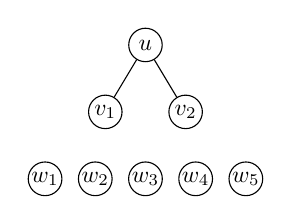
\begin{tikzpicture}[scale=0.85, every node/.style={scale=0.85,shape=circle,inner sep=.5pt,
                  minimum size=5mm}]
              \node[draw] (u) at (0,1) {$u$};
              \node[draw] (v1) at (-.6,0) {$v_1$};
              \node[draw] (v2) at (.6,0) {$v_2$};
              \node[draw] (w1) at (-1.5,-1) {$w_1$};
              \node[draw] (w2) at (-.75,-1) {$w_2$};
              \node[draw] (w3) at (0,-1) {$w_3$};
              \node[draw] (w4) at (.75,-1) {$w_4$};
              \node[draw] (w5) at (1.5,-1) {$w_5$};
              \draw (u) -- (v1);
              \draw (u) -- (v2);
          \end{tikzpicture}
        }
        \label{figure:gac-example-3}
    }
    \subfigure[][$H_2$] {
        \centering
        \scalebox{1}{
          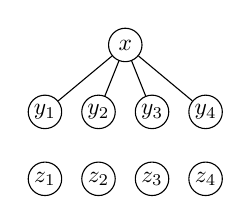
\begin{tikzpicture}[scale=0.85, every node/.style={scale=0.85,shape=circle,inner sep=.5pt,
                  minimum size=5mm}]
              \node[draw] (x) at (0,1) {$x$};
              \node[draw] (y1) at (-1.2,0) {$y_1$};
              \node[draw] (y2) at (-.4,0) {$y_2$};
              \node[draw] (y3) at (.4,0) {$y_3$};
              \node[draw] (y4) at (1.2,0) {$y_4$};
              \node[draw] (z1) at (-1.2,-1) {$z_1$};
              \node[draw] (z2) at (-.4,-1) {$z_2$};
              \node[draw] (z3) at (.4,-1) {$z_3$};
              \node[draw] (z4) at (1.2,-1) {$z_4$};
              \draw (x) -- (y1);
              \draw (x) -- (y2);
              \draw (x) -- (y3);
              \draw (x) -- (y4);
          \end{tikzpicture}
        }
        \label{figure:gac-example-4}
    }
    \subfigure[][$G_k$] {
        \centering
        \scalebox{1}{
          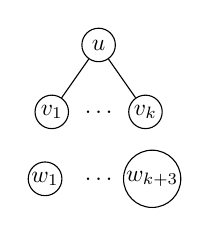
\begin{tikzpicture}[scale=0.85, every node/.style={scale=0.85,shape=circle,inner sep=.5pt,
                  minimum size=5mm}]
              \node[draw] (u) at (0,1) {$u$};
              \node[draw] (v1) at (-.7,0) {$v_1$};
              \node[] (vdots) at (0,0) {$\dots$};
              \node[draw] (v2) at (.7,0) {$v_k$};
              \node[draw] (w1) at (-.8,-1) {$w_1$};
              \node[] (wdots) at (0,-1) {$\dots$};
              \node[draw] (w5) at (.8,-1) {$w_{k+3}$};
              \draw (u) -- (v1);
              \draw (u) -- (v2);
          \end{tikzpicture}
        }
        \label{figure:gac-example-1}
    }
    \subfigure[][$H_k$] {
        \centering
        \scalebox{1}{
          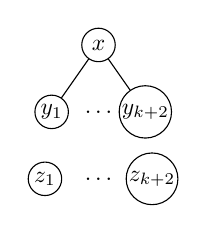
\begin{tikzpicture}[scale=0.85, every node/.style={scale=0.85,shape=circle,inner sep=.5pt,
                  minimum size=5mm}]
              \node[draw] (x) at (0,1) {$x$};
              \node[draw] (y1) at (-.7,0) {$y_1$};
              \node[] (ydots) at (0,0) {$\dots$};
              \node[draw] (y2) at (.7,0) {$y_{k+2}$};
              \node[draw] (z1) at (-.8,-1) {$z_1$};
              \node[] (zdots) at (0,-1) {$\dots$};
              \node[draw] (z5) at (.8,-1) {$z_{k+2}$};
              \draw (x) -- (y1);
              \draw (x) -- (y2);
          \end{tikzpicture}
        }
        \label{figure:gac-example-2}
    }
    \caption{Example graphs $G_2$ and $H_2$, and their generalised
    versions $G_k$ and $H_k$.}\label{figure:gac-example}
\end{figure}

When solving this instance, \McSplit-SI begins by mapping $u$ to $x$.  This leaves
two label classes:
$\langle \{v_1,v_2\}, \{y_1,y_2,y_3,y_4\} \rangle$
and
$\langle \{w_1,w_2,w_3,w_4,w_5\}, \{z_1,z_2,z_3,z_4\} \rangle$.  In the latter
label class, the set $V_G$ is larger than the set $V_H$, and therefore the
algorithm can backtrack and terminate.

Now we consider how the Glasgow algorithm behaves on this instance. After mapping
$u$ to $x$, the domains correspond to our label classes, as shown in the first two
columns of \Cref{tab:counting-all-diff}.  The remaining two columns of the table
illustrate the behaviour of the counting all-different propagator on these domains.
(Since all domains are of the same size, the stable sort function used by the algorithm
does not reorder the domains.)  The third column shows set $A$, which is the union
of domains in the current and previous rows.  The fourth column shows the number
of variables up to and including the current row.  Since $|A| \geq n$ on each row,
the propagator does not delete any values from the domains and does not conclude
that we can backtrack.

\begin{table}[h!]
\centering
\footnotesize
    \begin{tabular}{p{0.09\linewidth} p{0.16\linewidth} p{0.3\linewidth} p{0.08\linewidth}}
 \toprule
     Variable & Domain & $A$ & $n$\\ [0.5ex]
 \midrule
     $v_1$ & $\{y_1,y_2,y_3,y_4\}$ & $\{y_1,y_2,y_3,y_4\}$ & 1\\
     $v_2$ & $\{y_1,y_2,y_3,y_4\}$ & $\{y_1,y_2,y_3,y_4\}$ & 2\\
     $w_1$ & $\{z_1,z_2,z_3,z_4\}$ & $\{y_1,y_2,y_3,y_4,z_1,z_2,z_3,z_4\}$ & 3\\
     $w_2$ & $\{z_1,z_2,z_3,z_4\}$ & $\{y_1,y_2,y_3,y_4,z_1,z_2,z_3,z_4\}$ & 4\\
     $w_3$ & $\{z_1,z_2,z_3,z_4\}$ & $\{y_1,y_2,y_3,y_4,z_1,z_2,z_3,z_4\}$ & 5\\
     $w_4$ & $\{z_1,z_2,z_3,z_4\}$ & $\{y_1,y_2,y_3,y_4,z_1,z_2,z_3,z_4\}$ & 6\\
     $w_5$ & $\{z_1,z_2,z_3,z_4\}$ & $\{y_1,y_2,y_3,y_4,z_1,z_2,z_3,z_4\}$ & 7\\
%    $s_G$ & Pointer to Integer & Pointer to the first vertex of the $G$-set\\
%    \rule{0pt}{2.3ex}$e_G$ & Pointer to Integer & Pointer to one element past the last vertex of the $G$-set\\
 \bottomrule
\end{tabular}
\caption{A demonstration of the counting all-different propagator on $G_2$ and $H_2$
    after assigning $u$ to $x$.}
\label{tab:counting-all-diff}
\end{table}

The final two graphs in \Cref{figure:gac-example} generalise $G_2$ and $H_2$; as $k$ is incremented,
a vertex is added to each of the $v$, $w$, $y$ and $z$ sets.
\Cref{tab:gk-run-times} shows run times for the enumeration problem
using \McSplit-SI, Glasgow, Glasgow with no supplemental graphs, and RI for a range of values of $k$.
VF3 was excluded from the experiment because the current version does not handle disconnected graphs correctly.
\McSplit-SI solves the instance $k=1\,000\,000$ in less than a second;
Glasgow and RI time out on the $k=10$ and $k=6$ instances respectively.

\begin{table}[htb]
\centering
\footnotesize
    \begin{tabular}{r r r r r}
 \toprule
        $k$ & \McSplit-SI & Glasgow & Glasgow-NS& RI \\ % [0.5ex]
 \midrule
        3 &  0 &  0 &  0 &  2\\
        4 &  0 &  0 &  0 &  86\\
        5 &  0 &  2 &  2 &  4305\\
        6 &  0 &  21 &  19 &  *\\
        7 &  0 &  195 &  191 &  *\\
        8 &  0 &  2083 &  1966 &  *\\
        9 &  0 &  24254 &  23443 &  *\\
        10 &  0 &  * &  * &  *\\
        10000 &  6 & * & * & *\\
        100000 &  66 & * & * & *\\
        1000000 &  676 & * & * & *\\
 \bottomrule
\end{tabular}
\caption{Run times in ms for the induced subgraph isomorphism enumeration problem on $G_k$ and $H_k$.
    An asterisk indicates timeout at 100 seconds. Glasgow-NS is the Glasgow Subgraph Solver
    with supplemental graphs disabled.}
\label{tab:gk-run-times}
\end{table}

\subsection{A family of instances where \McSplit-SI is outperformed by Glasgow}

In the previous subsection, we saw a family of instances on which \McSplit-SI easily outperforms
the Glasgow Subgraph Solver.  We can easily construct a family of instances where the reverse is true.
Consider the graphs in \Cref{figure:glasgow-fast-example}.
Graph $G'_3$ consists of three copies of the cycle $C_4$ and three copies of the star
$K_{1,3}$, with no additional edges.  Graph $H'_3$ consists of three copies of $C_5$
and three copies of $K_{1,3}$.  We generalise these definition to $G'_k$ and $H'_k$,
which have $k$ copies the cycle and star rather than 3.
For $k\geq 1$, no instance $(G'_k, H'_k)$ is satisfiable, since $H'_k$ does not contain
an induced 4-cycle.

The \McSplit-SI algorithm prefers to map high-degree vertices first, and therefore its first
decisions on these instances involves the stars rather than the cycles.  Only at deeper
levels of the search
tree, when all of the stars have been mapped, does the algorithm begin to work on the cycles,
at which point it can backtrack.  Unfortunately, there are $6^k k!$ ways to map the stars
of $G'_k$ to the stars of $H'_k$, since any star in the pattern graph can be mapped to any
star in the target graph and there are six possible ways to map the leaf nodes of any star.
Therefore \McSplit-SI's search tree is very large even
for small values of $k$.

With supplemental graphs disabled, the Glasgow algorithm suffers from the same problem.
However, supplemental graphs allow the Glasgow Subgraph Solver to solve these instances
without search.  In particular, consider the supplemental graph in which $v$ and $w$
are adjacent
if and only there are at least two 2-paths between $v$ and $w$ in the original graph.
This supplemental graph
contains edges between vertices of the 4-cycles in the pattern graph, but has no edges for the
target graph.

\Cref{tab:gk-prime-run-times} shows that supplemental graphs make a huge
difference to Glasgow's run times in practice on this family of instances.  The
table shows times for \McSplit-SI, Glasgow, Glasgow without supplemental
graphs, and RI.  \McSplit-SI and RI have similar run times, and cannot solve
instances with $k$ greater than 5 within the 100 second time limit.  Glasgow can
solve the instance with $k=1000$ (a 7000-vertex pattern graph and an
8000-vertex target graph) in less than 4 seconds.

\begin{figure}[htb]
    \centering
    \subfigure[][$G'_3$] {
        \centering
        \scalebox{1}{
          \foreach \n in {1,...,3}{
              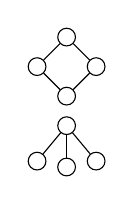
\begin{tikzpicture}[scale=0.75, every node/.style={scale=0.75,shape=circle,inner sep=.5pt,
                      minimum size=3mm}]
                  \node[draw] (a) at (0,0) {};
                  \node[draw] (b) at (.5,.5) {};
                  \node[draw] (c) at (1,0) {};
                  \node[draw] (d) at (.5,-.5) {};
                  \node[draw] (e) at (.5,-1) {};
                  \node[draw] (f) at (0,-1.6) {};
                  \node[draw] (g) at (.5,-1.7) {};
                  \node[draw] (h) at (1,-1.6) {};
                  \draw (a) -- (b) -- (c) -- (d) -- (a);
                  \draw (e) -- (f);
                  \draw (e) -- (g);
                  \draw (e) -- (h);
              \end{tikzpicture}
          }
        }
    }
    \subfigure[][$H'_3$] {
        \centering
        \scalebox{1}{
          \foreach \n in {1,...,3}{
              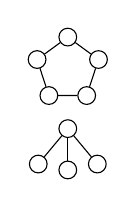
\begin{tikzpicture}[scale=0.75, every node/.style={scale=0.75,shape=circle,inner sep=.5pt,
                      minimum size=3mm}]
                  \node[draw] (z) at (0.5,0.55) {};
                  \node[draw] (a) at (-0.02,0.17) {};
                  \node[draw] (b) at (0.18,-0.44) {};
                  \node[draw] (c) at (0.82,-0.44) {};
                  \node[draw] (d) at (1.02,0.17) {};
                  \node[draw] (e) at (.5,-1) {};
                  \node[draw] (f) at (0,-1.6) {};
                  \node[draw] (g) at (.5,-1.7) {};
                  \node[draw] (h) at (1,-1.6) {};
                  \draw (a) -- (b) -- (c) -- (d) -- (z) -- (a);
                  \draw (e) -- (f);
                  \draw (e) -- (g);
                  \draw (e) -- (h);
              \end{tikzpicture}
          }
        }
    }
    \caption{Example graphs $G'_3$ and $H'_3$.}\label{figure:glasgow-fast-example}
\end{figure}

\begin{table}[htb]
\centering
\footnotesize
    \begin{tabular}{r r r r r}
 \toprule
     $k$ & \McSplit-SI & Glasgow & Glasgow-NS& RI \\ %[0.5ex]
 \midrule
     1 &  0 &  0 &  0 &  0\\
     2 &  0 &  0 &  1 &  0\\
     3 &  10 &  0 &  47 &  10\\
     4 &  329 &  0 &  1793 &  324\\
     5 &  12522 &  0 &  80880 &  11987\\
     6 &  * &  0 &  * &  *\\
     7 &  * &  0 &  * &  *\\
     8 &  * &  0 &  * &  *\\
     9 &  * &  0 &  * &  *\\
     10 &  * &  0 &  * &  *\\
     100 &  * &  27 &  * &  *\\
     1000 &  * &  3825 &  * &  *\\
 \bottomrule
\end{tabular}
\caption{Run times in ms for the induced subgraph isomorphism enumeration problem on $G'_k$ and $H'_k$.
    An asterisk indicates timeout at 100 seconds. Glasgow-NS is the Glasgow Subgraph Solver
    with supplemental graphs disabled.}
\label{tab:gk-prime-run-times}
\end{table}

As we have seen in this section, neither \McSplit-SI nor Glasgow dominates the other solver.  In the next
section, we perform an experimental evalulation to compare solvers on benchmark instances.

\FloatBarrier

\section{A version using linked lists of vertices}

The data structure used by \McSplit-SI to represent the two lists of vertices
within each label class enables fast partitioning, but has the disadvantage
that the vertices in each list are not kept in any particular order.  This has
two negative consequences.  First, when selecting a label class according to
the smallest domain first heuristic with degree-based tie breaking, we need to
scan the pattern-graph vertices within each label class of minimum size to find
a vertex of optimal degree.  Second, we face a time-space tradeoff when
iterating over the target-graph vertices in degree order on
\lineref{McSplitSIWLoop} of \Cref{McSplitSIAlg}: we can choose either to copy
the list of vertices representing $S_H$ and then sort this copy, or to scan the
list $S_H$ on each iteration for the next-best element.  The first of these
options --- which we use in our implementation --- requires $O(|S_H| \log
|S_H|)$ time and $n$ words of additional space; the second requires
$O(|S_H|^2)$ time and no additional space.

These disadvantages tend to be small in practice, as the label class chosen for
iteration tends to be small except at the root of the search tree.
Nevertheless, there exist pathological instances in which the smallest label
classes are large even deep in the search tree.  For example, if the pattern
and target graphs have no edges then there is only one label class at every
depth of recursion.  Therefore, it would be useful to have a version of
\McSplit-SI that keeps the vertices sorted in each label class without increasing
the time complexity of the partitioning procedure.  This section describes
such a version, which we call \McSplit-SI-LL because it stores lists of
vertices as doubly linked lists.

The data structures of \McSplit-SI-LL differ from those of \McSplit-SI
as follows.  \McSplit-SI-LL does not use the arrays \Garray\ and \Harray;
rather, each element of \Gptrs\ and \Hptrs\ has forward and backward pointers
that enable the vertices within a label class to be joined together as a linked list.
Since the linked-list nodes are embedded in an array, we can delete a given
vertex from a list in constant time in addition to the usual complexity
guarantees of doubly linked lists for other operations.  \Cref{figure:si-data-structures-ll-version}
shows the data structures of \McSplit-SI-LL after assigning vertex $1$ to vertex $a$;
this corresponds to \Cref{figure:si-data-structures} which shows the same state
using the data structures of \McSplit-SI.

\begin{figure}[htb]
    \centering
    \includegraphics*[width=0.9\textwidth]{14b-mcsplit-induced-si/figs/data-structure-step-1-ll-version}
    \caption{TODO}
    \label{figure:si-data-structures-ll-version}
\end{figure}

Before the first call to $\FuncSty{Search}()$, the two linked lists of vertices in
each label class are sorted in order of vertex degree.  We also sort each adjacency list
of graphs $G$ and $H$ in order of vertex degree.

We require the order to be maintained
by the $\FuncSty{Filter}$ and $\FuncSty{Unfilter}$ functions.  The first of these is straightforward:
when iterating over an adjacency list in the $\FuncSty{Filter}$ function, we delete each vertex $v$
from its label class and append it to the new label class.  Because the adjacency lists are sorted,
each new label class is in sorted order.

The $\FuncSty{Unfilter}$ function requires more work in \McSplit-SI-LL than in \McSplit-SI,
since when merging label classes we must ensure that each vertex is returned to the position
in its former label class from which it was removed.  To enable this, we perform a little extra
bookkeeping during the $\FuncSty{filter}$ function: each time we remove a vertex $v$, we store
$v$ in an array along with a pointer to its successor node in the linked list from which $v$
was removed.  TODO: say where we store these.

TODO (in pseudocode, not here): check if I'm updating label class pointers during filtering

In the next section, we will see that \McSplit-SI-LL is space-efficient.  The experimental evaluation
in the following section shows that \McSplit-SI-LL runs faster \McSplit-SI on some instances, but
slightly slower on many instances.

\FloatBarrier

\section{Space complexity}

The following proposition demonstrates that the memory needed by \McSplit-SI-LL
is bounded above by a constant multiple of the space used to store the adjacency
lists of $G$ and $H$.  While this is greater than the space complexity of 
VF3 and RI, which require only $|V(G)| + |V(H)|$ space, it is improvement
over all previous constraint programming algorithms, which
require at least $O(|V(G)| |V(H)|)$ space just to represent
the initial domains.  The Glasgow Subgraph Solver uses $O(|V(H)|)$ space
to represent adjacency matrices, and requires $O(|V(G)|^2|V(H)|)$ space
to solve any satisfiable instance.

\begin{proposition}\label{mcsplit-si-space}
    \McSplit-SI-LL uses $O(n_G + m_G + m_H)$ space, where
    $n_G=|V(G)|$,
    $m_G=|E(G)|$, and
    $m_H=|E(H)|$.
\end{proposition}

\begin{proof}
    The function $\FuncSty{Filter}(v,w)$ runs in $O(|N_G(v)| + |N_H(w)|)$ time
    and each of its operations allocates at most $O(1)$ space; therefore the
    function uses $O(|N_G(v)| + |N_H(w)|)$ space.

    Each of the functions
    $\FuncSty{SelectLabelClass}$,
    $\FuncSty{SelectVertex}$,
    $\FuncSty{Assign}$,
    $\FuncSty{Unassign}$,
    and
    $\FuncSty{Unfilter}$
    uses $O(1)$ space and does not allocate any memory that is not released
    when the function returns.  Moreover, $\FuncSty{Unfilter}$ releases
    all of the memory that was allocated by the corresponding call to $\FuncSty{Filter}$.

    The mapping $M$ can be no larger than $n_G$, so the maximum recursion depth for
    $\FuncSty{Search}$ calls is $n_G + 1$.  Now suppose we at the start of the
    $\FuncSty{Search}$ function at some given node at depth $k$ of the search tree 
    ($k \leq n_G + 1$).  At earlier levels of the call stack, $k-1$ calls to $\FuncSty{Filter}$
    have been made; the $v$ parameter for these calls has taken distinct values
    $\{v_1, \dots, v_{k-1}\} \subseteq V(G)$, and the $w$ parameter has taken distinct values
    $\{w_1, \dots, w_{k-1}\} \subseteq V(H)$.  These $\FuncSty{Filter}$ calls have used
    $\sum_{i=1}^{k-1} O(|N_G(v_i)| + |N_H(w_i)|) = O(m_G + m_H)$ space.  In total,
    local variables used in the $k$
    recursive calls of $FuncSty{Search}$ use a further $O(k) = O(n_G)$ space.  Thus,
    the total space usage is $O(n_G + m_G + m_H)$.
\end{proof}

\section{Experimental evaluation}

In this section, we compare the speed of \McSplit-SI with three state-of-the-art algorithms
on two sets of benchmark instances.  For the first set of instances, we solve the decision problem:
does there exist an induced subgraph isomorphism from the pattern graph to the target
graph?  For the second set of instances, we solve the problem of counting all induced subgraph
isomorphisms from the pattern to the target.

\subsection{Other solvers}

Our experiments compare \McSplit-SI with three state-of-the-art subgraph isomorphism solvers:
VF3, RI, and Glasgow.  

\paragraph*{Glasgow Subgraph Solver}
The Glasgow Subgraph Solver \cite{DBLP:conf/cp/McCreeshP15,DBLP:conf/gg/McCreeshP020}
(henceforth Glasgow)
was the fastest solver for hard induced subgraph isomorphism instances in a recent
experimental evaluation by Solnon \cite{DBLP:conf/gbrpr/Solnon19}.  The algorithm
uses a constraint programming approach, in which the domain of each vertex is represented
explicitly in memory.  Bitsets are used to represent domains and rows of each adjacency
matrix, allowing very fast updates to domains, particularly on dense graphs
\cite{ullmann1976algorithm}.  The Glasgow algorithm introduces the concept of
\emph{supplemental graphs}: graphs derived from the pattern and target graphs that
can also be used to filter domains.  This technique often results in a large
improvement to the solver's run time.  Unfortunately we cannot use the same technique
in \McSplit-SI because it breaks the invariant, required by \McSplit-SI's data structure,
that any two domains are either equal or disjoint.
We use the 14 March 2022 version of the Glasgow solver, published
online.\footnote{\url{https://github.com/ciaranm/glasgow-subgraph-solver}}
In addition, we report results of the Glasgow solver with supplemental graphs
switched off.

\paragraph*{VF3 and RI}
Like Glasgow, the VF3 \cite{DBLP:journals/pami/CarlettiFSV18} and RI
\cite{DBLP:journals/bmcbi/BonniciGPSF13,DBLP:journals/tcbb/BonniciG17}
solvers explore a search tree, adding one pair of vertices to the mapping at each
search node.  However, the data structures maintained by these algorithms are
much more lightweight than those of Glasgow.  VF3 and RI do not maintain
a domain for each vertex in the pattern graph; they simply store a partition
of the vertex set of each graph into three sets: ($A$) vertices that have been
mapped already, ($B$) unmapped vertices that are adjacent to at least one mapped vertex, and
($C$) all other unmapped vertices.
If the $B$ (resp. $C$) set of the target graph is smaller than the $B$ (resp. $C$)
set of the pattern graph, the algorithm can backtrack.
This data structure can be updated with the same
time complexity as the partitioning step of \McSplit-SI (and with a slightly
smaller constant factor given the simplicity of the data structure).  
However, its ability to prune the search tree is worse than that of \McSplit-SI
since the $B$ sets are a union of the label classes in \McSplit-SI, and it
leaves unavailable the smallest-domain-first heuristic used by \McSplit-SI.

(TODO mention RI-DS)

(TODO write about differences between VF3 and RI)

In terms of effort per search node, \McSplit-SI may be viewed intuitively as sitting
between Glasgow on one hand VF3 and RI on the other.

\paragraph*{\McSplit-SI-adjmat} Finally, we implemented a version of \McSplit\
for subgraph isomorphism that stores graphs as adjacency matrices rather than
adjacency lists.  This does not use the \McSplit-SI data structures described
in this chapter, and is essentially a decision version of the \McSplit\ solver
for maximum common subgraph described in \label{c:mcsplit-i-undirected}.
However, we tried to make the implementation fast, and indeed we will see in
the results that the algorithm often outperforms \McSplit-SI on instances with
relatively dense graphs.  The main additional feature compared to the maximum
common subgraph version of \McSplit is a version of the lazy partitioning
technique that was described in \Cref{subsec:lazy-partitioning}.  Before
running the partitioning algorithm, we iterate over the label classes, counting
in each label class the number of vertices adjacent to $v$ in the pattern graph
and to $w$ in the target class.  This often allows us to backtrack without the
need for the relatively expensive step of swapping vertices within a label
class.

\subsection{Decision instances}

\subsection{Families of instances}

\subsection{Results}

\begin{figure}[h!]
    \centering
    \subfigure[][Glasgow] {
        \includegraphics*[width=0.22\textwidth]{14b-mcsplit-induced-si/decision-instances-experiment/experiment/plots/cumulative-mcsplit-glasgow}
        \label{figure:TODO}
    }
    \subfigure[][Glasgow, no supp.] {
        \includegraphics*[width=0.22\textwidth]{14b-mcsplit-induced-si/decision-instances-experiment/experiment/plots/cumulative-mcsplit-glasgow-nosupp}
        \label{figure:TODO}
    }
    \subfigure[][RI] {
        \includegraphics*[width=0.22\textwidth]{14b-mcsplit-induced-si/decision-instances-experiment/experiment/plots/cumulative-mcsplit-ri}
        \label{figure:TODO}
    }
    \subfigure[][RI-DS] {
        \includegraphics*[width=0.22\textwidth]{14b-mcsplit-induced-si/decision-instances-experiment/experiment/plots/cumulative-mcsplit-ri-ds}
        \label{figure:TODO}
    }
    \subfigure[][VF3] {
        \includegraphics*[width=0.22\textwidth]{14b-mcsplit-induced-si/decision-instances-experiment/experiment/plots/cumulative-mcsplit-vf3}
        \label{figure:TODO}
    }
    \subfigure[][\McSplit-SI-LL] {
        \includegraphics*[width=0.22\textwidth]{14b-mcsplit-induced-si/decision-instances-experiment/experiment/plots/cumulative-mcsplit-si-ll}
        \label{figure:TODO}
    }
    \subfigure[][\McSplit-SI-AM] {
        \includegraphics*[width=0.22\textwidth]{14b-mcsplit-induced-si/decision-instances-experiment/experiment/plots/cumulative-mcsplit-si-am}
        \label{figure:TODO}
    }
    \caption{Cumulative plots of run times for decision instances.  In each subfigure, the algorithm named
        in the caption is in dark blue and \McSplit-SI is in light blue.}
    \label{figure:unlabelled-vf-instance-runtimes}
\end{figure}

\begin{figure}[h!]
    \centering
    \subfigure[][Glasgow] {
        \includegraphics*[width=0.22\textwidth]{14b-mcsplit-induced-si/decision-instances-experiment/experiment/plots/scatter-mcsplit-glasgow}
        \label{figure:TODO}
    }
    \subfigure[][Glasgow, no supp.] {
        \includegraphics*[width=0.22\textwidth]{14b-mcsplit-induced-si/decision-instances-experiment/experiment/plots/scatter-mcsplit-glasgow-nosupp}
        \label{figure:TODO}
    }
    \subfigure[][RI] {
        \includegraphics*[width=0.22\textwidth]{14b-mcsplit-induced-si/decision-instances-experiment/experiment/plots/scatter-mcsplit-ri}
        \label{figure:TODO}
    }
    \subfigure[][RI-DS] {
        \includegraphics*[width=0.22\textwidth]{14b-mcsplit-induced-si/decision-instances-experiment/experiment/plots/scatter-mcsplit-ri-ds}
        \label{figure:TODO}
    }
    \subfigure[][VF3] {
        \includegraphics*[width=0.22\textwidth]{14b-mcsplit-induced-si/decision-instances-experiment/experiment/plots/scatter-mcsplit-vf3}
        \label{figure:TODO}
    }
    \subfigure[][\McSplit-SI-LL] {
        \includegraphics*[width=0.22\textwidth]{14b-mcsplit-induced-si/decision-instances-experiment/experiment/plots/scatter-mcsplit-si-ll}
        \label{figure:TODO}
    }
    \subfigure[][\McSplit-SI-AM] {
        \includegraphics*[width=0.22\textwidth]{14b-mcsplit-induced-si/decision-instances-experiment/experiment/plots/scatter-mcsplit-si-am}
        \label{figure:TODO}
    }
    \caption{Scatter plots of run times for decision instances. TODO explain}
    \label{figure:unlabelled-vf-instance-runtimes-scatter}
\end{figure}

\begin{figure}[h!]
    \centering
    \subfigure[][Glasgow] {
        \includegraphics*[width=0.22\textwidth]{14b-mcsplit-induced-si/decision-instances-experiment/experiment/plots/scatter-presolve-mcsplit-glasgow}
        \label{figure:TODO}
    }
    \subfigure[][Glasgow, no supp.] {
        \includegraphics*[width=0.22\textwidth]{14b-mcsplit-induced-si/decision-instances-experiment/experiment/plots/scatter-presolve-mcsplit-glasgow-nosupp}
        \label{figure:TODO}
    }
    \subfigure[][RI] {
        \includegraphics*[width=0.22\textwidth]{14b-mcsplit-induced-si/decision-instances-experiment/experiment/plots/scatter-presolve-mcsplit-ri}
        \label{figure:TODO}
    }
    \subfigure[][RI-DS] {
        \includegraphics*[width=0.22\textwidth]{14b-mcsplit-induced-si/decision-instances-experiment/experiment/plots/scatter-presolve-mcsplit-ri-ds}
        \label{figure:TODO}
    }
    \subfigure[][VF3] {
        \includegraphics*[width=0.22\textwidth]{14b-mcsplit-induced-si/decision-instances-experiment/experiment/plots/scatter-presolve-mcsplit-vf3}
        \label{figure:TODO}
    }
    \subfigure[][\McSplit-SI-LL] {
        \includegraphics*[width=0.22\textwidth]{14b-mcsplit-induced-si/decision-instances-experiment/experiment/plots/scatter-presolve-mcsplit-si-ll}
        \label{figure:TODO}
    }
    \subfigure[][\McSplit-SI-AM] {
        \includegraphics*[width=0.22\textwidth]{14b-mcsplit-induced-si/decision-instances-experiment/experiment/plots/scatter-presolve-mcsplit-si-am}
        \label{figure:TODO}
    }
    \caption{Scatter plots of run times for decision instances with presolve. TODO explain}
    \label{figure:unlabelled-vf-instance-runtimes-scatter}
\end{figure}

TODO: mention that D1 variant isn't very good.
TODO: mention that D2 variant has similar results to Glasgow on phase instances.

\begin{table}[htb]
\centering
\footnotesize
    
\begin{tabular}{crrrrrrrr}
    \toprule
    Family & Count & McS-SI & McS-SI-LL & Gla & Gla, no supp. & RI & VF3 & McS pre.\\
    \midrule

1 & $100$ & $\underline{100}$ & $\underline{100}$ & $\underline{100}$ & $\underline{100}$ & $90$ & $98$ & $\underline{100}$\\
2 & $793$ & $\underline{793}$ & $\underline{793}$ & $789$ & $786$ & $708$ & $726$ & $791$\\
3 & $270$ & $\underline{270}$ & $\underline{270}$ & $\underline{270}$ & $\underline{270}$ & $\underline{270}$ & $\underline{270}$ & $\underline{270}$\\
4 & $270$ & $\underline{270}$ & $\underline{270}$ & $\underline{270}$ & $\underline{270}$ & $267$ & $269$ & $\underline{270}$\\
5 & $90$ & $89$ & $89$ & $\underline{90}$ & $\underline{90}$ & $\underline{90}$ & $87$ & $\underline{90}$\\
6 & $270$ & $\underline{270}$ & $\underline{270}$ & $\underline{270}$ & $\underline{270}$ & $\underline{270}$ & $\underline{270}$ & $\underline{270}$\\
7 & $270$ & $259$ & $259$ & $\underline{270}$ & $260$ & $263$ & $263$ & $\underline{270}$\\
9 & $24$ & $\underline{24}$ & $\underline{24}$ & $\underline{24}$ & $\underline{24}$ & $\underline{24}$ & $\underline{24}$ & $\underline{24}$\\
11 & $3\,038$ & $2\,939$ & $2\,938$ & $\underline{2\,967}$ & $2\,950$ & $2\,904$ & $2\,863$ & $2\,966$\\
12 & $200$ & $\underline{199}$ & $\underline{199}$ & $178$ & $179$ & $5$ & $4$ & $\underline{199}$\\
13 & $3\,018$ & $\underline{3\,018}$ & $\underline{3\,018}$ & $\underline{3\,018}$ & $\underline{3\,018}$ & $2\,781$ & $2\,914$ & $\underline{3\,018}$\\
14 & $6\,278$ & $\underline{6\,278}$ & $\underline{6\,278}$ & $\underline{6\,278}$ & $\underline{6\,278}$ & $\underline{6\,278}$ & $\underline{6\,278}$ & $\underline{6\,278}$\\
TOTAL & $14\,621$ & $14\,509$ & $14\,508$ & $14\,524$ & $14\,495$ & $13\,950$ & $14\,066$ & $\underline{14\,546}$\\

    \bottomrule
\end{tabular}


\caption{TODO solved counts}
\label{tab:TODO}
\end{table}

\begin{table}[htb]
\centering
\footnotesize
    
\begin{tabular}{crrrrrrrr}
    \toprule
    Family & Count & McS-SI & McS-SI-LL & Gla & Gla, no supp. & RI & VF3 & McS + pre.\\
    \midrule

1 & $100$ & $61$ & $48$ & $0$ & $0$ & $60$ & $39$ & $\underline{64}$\\
2 & $793$ & $651$ & $\underline{670}$ & $284$ & $379$ & $214$ & $220$ & $632$\\
3 & $270$ & $\underline{270}$ & $252$ & $0$ & $4$ & $\underline{270}$ & $230$ & $231$\\
4 & $270$ & $\underline{248}$ & $228$ & $0$ & $12$ & $221$ & $190$ & $217$\\
5 & $90$ & $\underline{67}$ & $62$ & $3$ & $0$ & $49$ & $5$ & $42$\\
6 & $270$ & $164$ & $159$ & $2$ & $0$ & $\underline{218}$ & $125$ & $161$\\
7 & $270$ & $128$ & $47$ & $12$ & $1$ & $31$ & $17$ & $\underline{171}$\\
9 & $24$ & $19$ & $19$ & $0$ & $0$ & $20$ & $18$ & $\underline{22}$\\
11 & $3\,038$ & $\underline{2\,464}$ & $2\,185$ & $730$ & $1\,066$ & $1\,838$ & $1\,435$ & $2\,369$\\
12 & $200$ & $\underline{198}$ & $1$ & $0$ & $0$ & $0$ & $0$ & $0$\\
13 & $3\,018$ & $\underline{3\,000}$ & $2\,884$ & $617$ & $1\,147$ & $2\,468$ & $1\,754$ & $2\,692$\\
14 & $6\,278$ & $4\,794$ & $4\,104$ & $0$ & $0$ & $4\,196$ & $3\,524$ & $\underline{5\,094}$\\
TOTAL & $14\,621$ & $\underline{12\,064}$ & $10\,659$ & $1\,648$ & $2\,609$ & $9\,585$ & $7\,557$ & $11\,695$\\

    \bottomrule
\end{tabular}


\caption{TODO winner counts}
\label{tab:TODO}
\end{table}

%% \begin{figure}[h!]
%%     \centering
%%     \includegraphics*[width=0.7\textwidth]{14b-mcsplit-induced-si/decision-instances-experiment/experiment/plots/cumulative-presolve}
%%     \caption{cumulative-presolve}
%%     \label{figure:cumulative-presolve}
%% \end{figure}
%% 
%% \begin{figure}[h!]
%%     \centering
%%     \includegraphics*[width=0.7\textwidth]{14b-mcsplit-induced-si/decision-instances-experiment/experiment/plots/cumulative}
%%     \caption{cumulative}
%%     \label{figure:cumulative}
%% \end{figure}
%% 
%% \begin{figure}[h!]
%%     \centering
%%     \includegraphics*[width=0.7\textwidth]{14b-mcsplit-induced-si/decision-instances-experiment/experiment/plots/sat-cumulative}
%%     \caption{sat-cumulative}
%%     \label{figure:sat-cumulative}
%% \end{figure}
%% 
%% \begin{figure}[h!]
%%     \centering
%%     \includegraphics*[width=0.7\textwidth]{14b-mcsplit-induced-si/decision-instances-experiment/experiment/plots/unsat-cumulative}
%%     \caption{unsat-cumulative}
%%     \label{figure:unsat-cumulative}
%% \end{figure}
%% 
%% \begin{figure}[h!]
%%     \centering
%%     \includegraphics*[width=0.7\textwidth]{14b-mcsplit-induced-si/decision-instances-experiment/experiment/plots/cumulative-without-disconnected-instances}
%%     \caption{cumulative-without-disconnected-instances}
%%     \label{figure:cumulative-without-disconnected-instances}
%% \end{figure}
%% 
%% \begin{figure}[h!]
%%     \centering
%%     \includegraphics*[width=0.45\textwidth]{14b-mcsplit-induced-si/decision-instances-experiment/experiment/plots/mcsplit-si-vs-adjmat}
%%     \caption{mcsplit-si-vs-adjmat}
%%     \label{figure:mcsplit-si-vs-adjmat}
%% \end{figure}
%% 
%% \begin{figure}[h!]
%%     \centering
%%     \includegraphics*[width=0.45\textwidth]{14b-mcsplit-induced-si/decision-instances-experiment/experiment/plots/mcsplit-si-vs-ll}
%%     \caption{mcsplit-si-vs-ll}
%%     \label{figure:mcsplit-si-vs-ll}
%% \end{figure}
%% 
%% \begin{figure}[h!]
%%     \centering
%%     \includegraphics*[width=0.45\textwidth]{14b-mcsplit-induced-si/decision-instances-experiment/experiment/plots/mcsplit-si-vs-glasgow}
%%     \caption{mcsplit-si-vs-glasgow}
%%     \label{figure:mcsplit-si-vs-glasgow}
%% \end{figure}
%% 
%% \begin{figure}[h!]
%%     \centering
%%     \includegraphics*[width=0.45\textwidth]{14b-mcsplit-induced-si/decision-instances-experiment/experiment/plots/mcsplit-si-domstatic-vs-glasgow}
%%     \caption{mcsplit-si-vs-glasgow}
%%     \label{figure:mcsplit-si-vs-glasgow}
%% \end{figure}
%% 
%% \begin{figure}[h!]
%%     \centering
%%     \includegraphics*[width=0.45\textwidth]{14b-mcsplit-induced-si/decision-instances-experiment/experiment/plots/mcsplit-si-vs-vf3}
%%     \caption{mcsplit-si-vs-vf3}
%%     \label{figure:mcsplit-si-vs-vf3}
%% \end{figure}

\FloatBarrier

\subsection{Knight's grid instances}

Our second set of decision-problem instances were proposed by Knuth in a recent pre-fascicle
of The Art of Computer Programming \cite{knuth2022art}.  Each pattern graph is a rectangular grid
$P_m \square P_n$, and each target graph is a knight graph $N_t$ which has one vertex for each
square of a $t \times t$ chessboard and an edge between any two squares that are a knight's
move (two squares horizontally and one square vertically or vice versa) apart.
\Cref{figure:knights-example} shows one of these instances and a solution.

\begin{figure}[htb]
    \centering
    \subfigure[][The grid $P_2 \square P_{24}$] {
        \centering
        \includegraphics*[width=0.36\textwidth]{14b-mcsplit-induced-si/knight-grid-experiment/img/p2-p24.pdf}
        \label{figure:grid-p2-p24}
    }
    \subfigure[][The knight graph $N_{12}$] {
        \centering
        \includegraphics*[width=0.36\textwidth]{14b-mcsplit-induced-si/knight-grid-experiment/img/12-by-12-p2-p24.pdf}
        \label{figure:knight12}
    }
    \caption{A satisfiable knight's grid instance. On the left is the pattern graph; on the right
            is the target graph with an induced subgraph isomorphic to the pattern shown by heavy
            nodes and edges.}\label{figure:knights-example}
\end{figure}

If $m=1$ and $n=t^2$, we have the classic knight's tour problem in which a single knight
must visit every square of the chessboard without revisiting any square.  The instances proposed
by Knuth have $m \in \{2,3,4\}$.  These instances may be interpreted as the problem of moving $m$
knights --- themselves organised in the formation of a miniature knight's tour of length $m$ ---
around the board without changing their positions relative to each other, and without revisiting
any square.  In the induced case (which is the only case we consider in this chapter), there
is the additional restriction that no knight attacks any square except the square that it has
just visited, the square it will visit next, and the squares of its neighbours in the miniature
tour of length $m$.

\begin{table}[htb]
\centering
\footnotesize
    
\begin{tabular}{ccrrrrrr}
    \toprule
    {$G$} & {$H$} & {McS-SI} & {McS-SI-LL} & {McS-SI-am} & Glasgow & RI-DS & VF3\\ 
    \midrule

$P_2\square P_{10}$ & $K_{8}$ & $\underline{0}$ & $\underline{0}$ & $\underline{0}$ & $2$ & $\underline{0}$ & $\underline{0}$\\
$P_2\square P_{12}$ & $K_{9}$ & $1$ & $1$ & $2$ & $2$ & $1$ & $\underline{0}$\\
$P_2\square P_{15}$ & $K_{10}$ & $12$ & $\underline{9}$ & $16$ & $96$ & $15$ & $29$\\
$P_2\square P_{19}$ & $K_{11}$ & $25$ & $20$ & $34$ & $657$ & $21$ & $\underline{0}$\\
$P_2\square P_{24}$ & $K_{12}$ & $6\,064$ & $4\,823$ & $8\,751$ & $22\,606$ & $\underline{143}$ & $209$\\
$P_2\square P_{28}$ & $K_{13}$ & $8\,244$ & $6\,292$ & $12\,092$ & $60\,227$ & $\underline{1\,011}$ & $2\,280$\\
$P_2\square P_{32}$ & $K_{14}$ & $3\,764$ & $2\,785$ & $5\,455$ & $\underline{1\,908}$ & $69\,164$ & $158\,409$\\
$P_2\square P_{36}$ & $K_{15}$ & $5\,121\,895$ & $3\,866\,617$ & $7\,825\,426$ & * & $50\,529$ & $\underline{2}$\\
$P_2\square P_{40}$ & $K_{16}$ & $726\,421$ & $528\,770$ & $1\,097\,532$ & * & $27\,932$ & $\underline{9\,641}$\\
$P_2\square P_{46}$ & $K_{17}$ & $9\,458\,240$ & $\underline{6\,858\,293}$ & * & * & * & *\\
$P_2\square P_{52}$ & $K_{18}$ & * & * & * & * & * & *\\

    \bottomrule
\end{tabular}


\caption{TODO SAT 2}
\label{tab:TODO}
\end{table}

\begin{table}[htb]
\centering
\footnotesize
    
\begin{tabular}{ccrrrrrrr}
    \toprule
    {$G$} & {$H$} & {McS-SI} & {McS-SI-LL} & {McS-SI-am} & Glasgow & RI-DS & VF3 & pathLAD \\ 
    \midrule

$P_3\square P_{7}$ & $K_{9}$ & $\underline{1}$ & $\underline{1}$ & $\underline{1}$ & $\underline{1}$ & $\underline{1}$ & $15$ & $9$\\
$P_3\square P_{10}$ & $K_{10}$ & $15$ & $12$ & $35$ & $25$ & $\underline{4}$ & $444$ & $31$\\
$P_3\square P_{11}$ & $K_{11}$ & $210$ & $213$ & $289$ & $145$ & $\underline{7}$ & $2\,730$ & $85$\\
$P_3\square P_{12}$ & $K_{12}$ & $43$ & $37$ & $69$ & $15$ & $\underline{9}$ & $16\,154$ & $106$\\
$P_3\square P_{14}$ & $K_{13}$ & $147$ & $94$ & $240$ & $174$ & $\underline{23}$ & $333\,160$ & $245$\\
$P_3\square P_{16}$ & $K_{14}$ & $22$ & $\underline{11}$ & $21$ & $320$ & $367$ & * & $4\,945$\\
$P_3\square P_{20}$ & $K_{15}$ & $30$ & $\underline{27}$ & $31$ & $65$ & $140$ & * & $1\,459$\\
$P_3\square P_{21}$ & $K_{16}$ & $7$ & $\underline{6}$ & $13$ & $7$ & $114$ & * & $1\,725$\\
$P_3\square P_{25}$ & $K_{17}$ & $192$ & $\underline{98}$ & $366$ & $616$ & $193$ & * & $4\,083$\\
$P_3\square P_{28}$ & $K_{18}$ & $1\,711$ & $1\,493$ & $3\,200$ & $\underline{356}$ & $374$ & * & $9\,891$\\
$P_3\square P_{32}$ & $K_{19}$ & $4\,720$ & $4\,217$ & $9\,270$ & $9\,508$ & $\underline{688}$ & * & $26\,583$\\
$P_3\square P_{34}$ & $K_{20}$ & $22\,382$ & $20\,370$ & $44\,440$ & $50\,447$ & $\underline{2\,033}$ & * & $74\,184$\\
$P_3\square P_{41}$ & $K_{21}$ & * & * & * & $634\,110$ & $\underline{149\,497}$ & * & $2\,093\,761$\\
$P_3\square P_{44}$ & $K_{22}$ & $452\,414$ & $\underline{411\,407}$ & $949\,089$ & * & $866\,380$ & * & *\\
$P_3\square P_{49}$ & $K_{23}$ & * & * & * & * & * & * & *\\

    \bottomrule
\end{tabular}


\caption{TODO SAT 3}
\label{tab:TODO}
\end{table}

\begin{table}[htb]
\centering
\footnotesize
    
\begin{tabular}{ccrrrrrrr}
    \toprule
    {$G$} & {$H$} & {McS-SI} & {McS-SI-LL} & {McS-SI-am} & Glasgow & RI-DS & VF3 & pathLAD \\ 
    \midrule

$P_4\square P_{8}$ & $K_{10}$ & $2$ & $\underline{1}$ & $2$ & $15$ & $2$ & $3$ & $20$\\
$P_4\square P_{8}$ & $K_{11}$ & $\underline{0}$ & $\underline{0}$ & $\underline{0}$ & $5$ & $4$ & $\underline{0}$ & $16$\\
$P_4\square P_{10}$ & $K_{12}$ & $5$ & $\underline{3}$ & $6$ & $4$ & $16$ & $71$ & $149$\\
$P_4\square P_{12}$ & $K_{13}$ & $31$ & $27$ & $37$ & $\underline{6}$ & $81$ & $925$ & $531$\\
$P_4\square P_{12}$ & $K_{14}$ & $5$ & $\underline{4}$ & $11$ & $5$ & $79$ & $797$ & $324$\\
$P_4\square P_{14}$ & $K_{15}$ & $\underline{3}$ & $\underline{3}$ & $4$ & $9$ & $63$ & $829$ & $200$\\
$P_4\square P_{15}$ & $K_{16}$ & $46$ & $\underline{41}$ & $53$ & $177$ & $73$ & $6\,620$ & $805$\\
$P_4\square P_{17}$ & $K_{17}$ & $128$ & $\underline{80}$ & $232$ & $205$ & $738$ & $137\,528$ & $6\,441$\\
$P_4\square P_{18}$ & $K_{18}$ & $2\,164$ & $2\,024$ & $4\,631$ & $\underline{861}$ & $34\,949$ & $7\,272\,239$ & $171\,695$\\
$P_4\square P_{20}$ & $K_{19}$ & $853$ & $\underline{813}$ & $1\,196$ & $1\,317$ & $12\,148$ & * & $61\,331$\\
$P_4\square P_{20}$ & $K_{20}$ & $53$ & $\underline{49}$ & $117$ & $394$ & $16\,241$ & $5\,612\,600$ & $44\,175$\\
$P_4\square P_{22}$ & $K_{21}$ & $644$ & $\underline{616}$ & $1\,604$ & $909$ & $47\,454$ & * & $129\,532$\\
$P_4\square P_{24}$ & $K_{22}$ & $15\,511$ & $\underline{13\,632}$ & $37\,208$ & $83\,256$ & $2\,199\,540$ & * & $2\,276\,484$\\
$P_4\square P_{25}$ & $K_{23}$ & $4\,091$ & $\underline{3\,659}$ & $12\,321$ & $5\,010$ & $1\,105\,560$ & * & $73\,827$\\
$P_4\square P_{26}$ & $K_{24}$ & $6\,686$ & $6\,772$ & $18\,261$ & $\underline{971}$ & $1\,761\,964$ & * & $660\,051$\\
$P_4\square P_{28}$ & $K_{25}$ & $4\,669$ & $4\,342$ & $15\,783$ & $\underline{938}$ & * & * & $270\,330$\\
$P_4\square P_{29}$ & $K_{26}$ & $15\,680$ & $\underline{14\,270}$ & $47\,237$ & $380\,938$ & * & * & $5\,051\,750$\\
$P_4\square P_{31}$ & $K_{27}$ & $248\,356$ & $\underline{224\,468}$ & $801\,511$ & $1\,784\,939$ & * & * & *\\
$P_4\square P_{32}$ & $K_{28}$ & $27\,628$ & $\underline{25\,833}$ & $108\,558$ & $1\,616\,244$ & * & * & $2\,321\,130$\\
$P_4\square P_{34}$ & $K_{29}$ & $141\,654$ & $\underline{127\,916}$ & $574\,230$ & $334\,914$ & * & * & *\\
$P_4\square P_{35}$ & $K_{30}$ & $147\,499$ & $131\,701$ & $583\,768$ & $\underline{19\,584}$ & * & * & *\\
$P_4\square P_{37}$ & $K_{31}$ & * & * & * & $\underline{122\,853}$ & * & * & *\\
$P_4\square P_{38}$ & $K_{32}$ & * & * & * & $\underline{6\,734\,566}$ & * & * & *\\
$P_4\square P_{40}$ & $K_{33}$ & * & * & * & * & * & * & *\\

    \bottomrule
\end{tabular}


\caption{TODO SAT 4}
\label{tab:TODO}
\end{table}

\begin{table}[htb]
\centering
\footnotesize
    
\begin{tabular}{ccrrrrrrr}
    \toprule
    {$G$} & {$H$} & {McS-SI} & {McS-SI-LL} & {McS-SI-am} & Glasgow & RI-DS & VF3 & pathLAD \\ 
    \midrule

$P_2\square P_{9}$ & $K_{6}$ & $\underline{1}$ & $\underline{1}$ & $2$ & $3$ & $2$ & $4$ & $14$\\
$P_2\square P_{9}$ & $K_{7}$ & $4$ & $\underline{3}$ & $9$ & $15$ & $11$ & $25$ & $66$\\
$P_2\square P_{11}$ & $K_{8}$ & $13$ & $\underline{11}$ & $17$ & $52$ & $38$ & $84$ & $159$\\
$P_2\square P_{13}$ & $K_{9}$ & $50$ & $\underline{41}$ & $66$ & $126$ & $147$ & $337$ & $680$\\
$P_2\square P_{16}$ & $K_{10}$ & $330$ & $\underline{281}$ & $455$ & $1\,049$ & $738$ & $1\,670$ & $5\,491$\\
$P_2\square P_{20}$ & $K_{11}$ & $1\,673$ & $\underline{1\,376}$ & $2\,146$ & $5\,979$ & $3\,641$ & $8\,267$ & $30\,007$\\
$P_2\square P_{25}$ & $K_{12}$ & $5\,692$ & $\underline{4\,839}$ & $8\,250$ & $24\,484$ & $21\,866$ & $40\,070$ & $100\,831$\\
$P_2\square P_{29}$ & $K_{13}$ & $31\,851$ & $\underline{27\,071}$ & $49\,951$ & $147\,194$ & $138\,465$ & $290\,711$ & $630\,856$\\
$P_2\square P_{33}$ & $K_{14}$ & $528\,697$ & $\underline{446\,389}$ & $748\,694$ & $2\,870\,431$ & $1\,564\,256$ & $3\,208\,128$ & $7\,911\,484$\\
$P_2\square P_{37}$ & $K_{15}$ & $8\,437\,193$ & $\underline{7\,151\,381}$ & * & * & * & * & *\\
$P_2\square P_{41}$ & $K_{16}$ & * & * & * & * & * & * & *\\

    \bottomrule
\end{tabular}


\caption{TODO UNSAT 2}
\label{tab:TODO}
\end{table}

\begin{table}[htb]
\centering
\footnotesize
    
\begin{tabular}{ccrrrrrrr}
    \toprule
    {$G$} & {$H$} & {McS-SI} & {McS-SI-LL} & {McS-SI-AM} & Glasgow & RI-DS & VF3 & pathLAD \\ 
    \midrule

$P_3\square P_{6}$ & $K_{7}$ & $2$ & $\underline{1}$ & $3$ & $3$ & $6$ & $11$ & $22$\\
$P_3\square P_{7}$ & $K_{8}$ & $8$ & $\underline{6}$ & $20$ & $16$ & $26$ & $152$ & $149$\\
$P_3\square P_{8}$ & $K_{9}$ & $\underline{21}$ & $31$ & $34$ & $37$ & $53$ & $475$ & $313$\\
$P_3\square P_{11}$ & $K_{10}$ & $111$ & $\underline{57}$ & $105$ & $165$ & $149$ & $35\,515$ & $1\,715$\\
$P_3\square P_{12}$ & $K_{11}$ & $207$ & $\underline{145}$ & $331$ & $418$ & $325$ & $117\,455$ & $4\,047$\\
$P_3\square P_{13}$ & $K_{12}$ & $334$ & $\underline{298}$ & $549$ & $755$ & $752$ & $787\,874$ & $7\,312$\\
$P_3\square P_{15}$ & $K_{13}$ & $569$ & $\underline{521}$ & $1\,032$ & $1\,622$ & $2\,046$ & * & $19\,247$\\
$P_3\square P_{17}$ & $K_{14}$ & $1\,195$ & $\underline{1\,114}$ & $2\,186$ & $3\,913$ & $4\,807$ & * & $45\,530$\\
$P_3\square P_{21}$ & $K_{15}$ & $2\,243$ & $\underline{1\,946}$ & $4\,811$ & $10\,312$ & $10\,606$ & * & $135\,926$\\
$P_3\square P_{22}$ & $K_{16}$ & $5\,924$ & $\underline{5\,196}$ & $11\,880$ & $26\,097$ & $36\,063$ & * & $308\,735$\\
$P_3\square P_{26}$ & $K_{17}$ & $51\,315$ & $\underline{44\,537}$ & $93\,507$ & $357\,274$ & $112\,509$ & * & $4\,808\,239$\\
$P_3\square P_{29}$ & $K_{18}$ & $144\,216$ & $\underline{126\,328}$ & $277\,555$ & $1\,046\,587$ & $371\,839$ & * & *\\
$P_3\square P_{33}$ & $K_{19}$ & $372\,099$ & $\underline{325\,976}$ & $770\,761$ & $2\,485\,598$ & $1\,524\,389$ & * & *\\
$P_3\square P_{35}$ & $K_{20}$ & $3\,752\,402$ & $\underline{3\,279\,381}$ & $7\,163\,297$ & * & $8\,555\,073$ & * & *\\
$P_3\square P_{42}$ & $K_{21}$ & * & * & * & * & * & * & *\\

    \bottomrule
\end{tabular}


\caption{TODO UNSAT 3}
\label{tab:TODO}
\end{table}

\begin{table}[htb]
\centering
\footnotesize
    
\begin{tabular}{ccrrrrrrr}
    \toprule
    {$G$} & {$H$} & {McS-SI} & {McS-SI-LL} & {McS-SI-AM} & Glasgow & RI-DS & VF3 & pathLAD \\ 
    \midrule

$P_4\square P_{5}$ & $K_{7}$ & $\underline{1}$ & $\underline{1}$ & $\underline{1}$ & $4$ & $6$ & $12$ & $33$\\
$P_4\square P_{6}$ & $K_{8}$ & $4$ & $\underline{3}$ & $6$ & $15$ & $18$ & $31$ & $75$\\
$P_4\square P_{7}$ & $K_{9}$ & $9$ & $\underline{8}$ & $16$ & $24$ & $47$ & $143$ & $223$\\
$P_4\square P_{9}$ & $K_{10}$ & $32$ & $\underline{27}$ & $54$ & $140$ & $156$ & $510$ & $921$\\
$P_4\square P_{9}$ & $K_{11}$ & $84$ & $\underline{72}$ & $182$ & $244$ & $375$ & $1\,402$ & $2\,128$\\
$P_4\square P_{11}$ & $K_{12}$ & $243$ & $\underline{209}$ & $395$ & $572$ & $803$ & $6\,507$ & $6\,338$\\
$P_4\square P_{13}$ & $K_{13}$ & $417$ & $\underline{395}$ & $750$ & $1\,284$ & $1\,903$ & $24\,227$ & $11\,657$\\
$P_4\square P_{13}$ & $K_{14}$ & $829$ & $\underline{682}$ & $1\,560$ & $2\,778$ & $4\,894$ & $70\,695$ & $25\,875$\\
$P_4\square P_{15}$ & $K_{15}$ & $1\,834$ & $\underline{1\,524}$ & $3\,451$ & $7\,277$ & $13\,036$ & $557\,027$ & $102\,684$\\
$P_4\square P_{16}$ & $K_{16}$ & $3\,001$ & $\underline{2\,620}$ & $6\,402$ & $13\,878$ & $33\,982$ & $2\,016\,052$ & $143\,635$\\
$P_4\square P_{18}$ & $K_{17}$ & $6\,700$ & $\underline{5\,700}$ & $13\,302$ & $34\,386$ & $92\,317$ & * & $492\,191$\\
$P_4\square P_{19}$ & $K_{18}$ & $17\,405$ & $\underline{16\,800}$ & $36\,632$ & $107\,312$ & $309\,409$ & * & $1\,792\,279$\\
$P_4\square P_{21}$ & $K_{19}$ & $36\,909$ & $\underline{33\,449}$ & $84\,628$ & $251\,562$ & $1\,081\,308$ & * & $3\,937\,353$\\
$P_4\square P_{21}$ & $K_{20}$ & $87\,626$ & $\underline{78\,268}$ & $200\,288$ & $576\,556$ & $2\,996\,995$ & * & $9\,786\,249$\\
$P_4\square P_{23}$ & $K_{21}$ & $219\,394$ & $\underline{196\,354}$ & $522\,896$ & $1\,609\,817$ & * & * & *\\
$P_4\square P_{25}$ & $K_{22}$ & $145\,464$ & $\underline{133\,384}$ & $430\,028$ & $922\,425$ & * & * & $5\,036\,360$\\
$P_4\square P_{26}$ & $K_{23}$ & $1\,111\,894$ & $\underline{988\,298}$ & $2\,944\,771$ & $7\,615\,315$ & * & * & *\\
$P_4\square P_{27}$ & $K_{24}$ & $1\,717\,197$ & $\underline{1\,555\,701}$ & $5\,220\,754$ & * & * & * & *\\
$P_4\square P_{29}$ & $K_{25}$ & $7\,288\,774$ & $\underline{6\,578\,751}$ & * & * & * & * & *\\
$P_4\square P_{30}$ & $K_{26}$ & * & * & * & * & * & * & *\\

    \bottomrule
\end{tabular}


\caption{TODO UNSAT 4}
\label{tab:TODO}
\end{table}

TODO talk about structure of instances (regular, symmetric, sparse) and give at least one run
time of Knuth's program.

\FloatBarrier

\subsection{Enumeration instances}

Our final set of benchmark instances is based on the MIVIA LDGraphs dataset
\cite{DBLP:journals/pami/CarlettiFSV18}.  In each LDGraphs instance, the pattern and
target graphs are random directed graphs with vertex labels but without edge labels.
Although the results of benchmarking graph algorithms on such instances cannot
always be extrapolated to real-world instances \cite{DBLP:conf/cp/McCreeshPST17},
we include these instances because they are the an established benchmark set,
and in particular they are the main set of instances used to demonstrate the
performance of VF3.

Rather than using the instance files provided by the authors of the MIVIA LDGraphs
dataset, we chose to generate our own random graphs from the same model and with the
same parameters.  We made this choice for two reasons: first, because of the large size
of the LDGraphs files (90 GBytes compressed), and second, so that we could add sparser
instances to the set of instances.

In each instance, both the pattern and target graph are generated using a directed-graph
version of the Erd\H{o}s-Rényi $G(n,p)$ model.  In this model, a graph on $n$ vertices
is generated, and each of the $n(n-1)$ possible directed edges is added with independent
probability $p$.  Carletti et al.\ use the values $\{0.2, 0.3, 0.4\}$ for $p$. In our experiment
we additionally use the values $0.05$ and $0.1$.

Following Carletti et al., we generate two families of directed graphs: an unlabelled family
and a family with no edge labels in which the vertex labels are chosen uniformly at random
from the set $\{1,\dots,8\}$.  (Carletti et al.\ generated a third family, in which labels
are chosen from a non-uniform distribution.  Their experimental results show very similar
outcomes for the uniform and non-uniform families, and therefore we have omitted the non-uniform
family from our experiment.)

For each value of $p$, we use the values
of $n$ for the target graph that were used by Carletti et al.; these are shown in \Cref{tab:carletti-n}.
In each instance, a randomly-selected subset of $20\%$ of the target vertices is selected,
and the subgraph induced by this subset is used as the pattern graph.

We do not include the LAD solver in our experiments because
the experimental results of \cite{DBLP:journals/pami/CarlettiFSV18} show that LAD
is orders of magnitude slower than VF3 on instances constructed in
this way.

\begin{table}[h!]
\centering
\footnotesize
 \begin{tabular}{p{0.2\linewidth} p{0.35\linewidth} p{0.35\linewidth}}
 \toprule
     $p$ & Target graph $n$ (unlabelled) & Target graph $n$ (labelled) \\ [0.5ex]
 \midrule
     $0.05$, $0.01$, and $0.2$ &
         300, 500, 750, 1000, 1250, 1500, 2000, 2500, 3000, 3500, 4000, 4500, 5000 &
         300, 500, 750, 1000, 1250, 1500, 2000, 2500, 3000, 3500, 4000, 4500, 5000,
         5500, 6000, 6500, 7000, 7500, 8000, 9000, 10000\\
     \rule{0pt}{2.3ex}$0.3$ & 
        300, 500, 750, 1000, 1250, 1500, 2000, 2500, 3000 &
        300, 500, 750, 1000, 1250, 1500, 2000, 2500, 3000, 3500, 4000, 4500, 5000,
        5500, 6000, 6500, 7000, 7500, 8000, 9000 \\
     \rule{0pt}{2.3ex}$0.4$ & 300, 500, 750, 1000, 1250, 1500 &
        300, 500, 750, 1000, 1250, 1500, 2000, 2500, 3000, 3500, 4000, 4500, 5000, 5500, 6000, 6500, 7000 \\
 \bottomrule
\end{tabular}
\caption{Values of $n$ used in enumeration instances}
\label{tab:carletti-n}
\end{table}

\FloatBarrier

\subsection{Results for unlabelled instances}

\Cref{figure:unlabelled-vf-instance-runtimes} shows run times for the unlabelled instances.
Since the instances have a natural ordering by the parameter $n$, we follow the example
of \cite{DBLP:journals/pami/CarlettiFSV18} and plot average run time as a function of $n$
rather than using cumulative plots.
Each point shows, for a given solver and given values of $n$ and $p$, the arithmetic mean of
run time in milliseconds for the 10 instances.
The time limit was set to 10000 seconds because many of the larger instances in this experiment
are particularly challenging.  Runs that exceeded the time limit were counted as taking 10000 seconds;
since none of the \McSplit-SI runs timed out, this does not affect the \McSplit-SI results but biases
the results slightly in favour of the other algorithms.  In cases where all ten runs timed out,
the data point is omitted from the plot (as, for example,  is the case for RI with $p=0.4$ and $n=7000$).

For all five values of $p$, either \McSplit-SI or \McSplit-SI-AM is the fastest algorithm.  For
the smallest two values of $p$, \McSplit-SI is the winner; for $p=0.2$ and above, \McSplit-SI-AM
is slightly faster.  This is as we would expect, since \McSplit-SI is designed to work well
on instances with sparse pattern and target graphs.  
\McSplit-SI-LL typically takes around two to three times as long as \McSplit-SI to find all solutions.

For each value of $p$, there is approximately an order of magnitude difference in run time between
the fastest variant of \McSplit-SI and the fastest non-\McSplit-SI algorithm.
On sparser instances, VF3 and RI-DS have the closest run times to \McSplit-SI.  Around $p=0.1$,
the Glasgow solver with supplemental graphs disabled becomes competitive with these algorithm, and at $p=0.4$
it is at least an order of magnitude faster than either VF3 or RI-DS.

When using the Glasgow solver, it is worthwhile to disable supplemental graphs
on all but 11 of the instances.  In fact, supplemental graphs have no effect on
the size of the search tree on the majority of instances, since most pairs of
vertices in this set of instances are joined by many paths of length 2; thus,
on this set of instances supplemental graphs have a double overhead --- in
their construction and in their use during search --- with no corresponding
benefit.

\begin{figure}[h!]
    \centering
    \subfigure[][Key] {
        \includegraphics*[trim=-40 -30 -40 -30,width=0.44\textwidth]{14b-mcsplit-induced-si/vf3-instances-experiment/experiment/plots/key.pdf}
        \label{figure:TODO}
    }
    \subfigure[][$p=0.05$] {
        \includegraphics*[width=0.44\textwidth]{14b-mcsplit-induced-si/vf3-instances-experiment/experiment/plots/runtimes0.05-1.pdf}
        \label{figure:TODO}
    }
    \subfigure[][$p=0.1$] {
        \includegraphics*[width=0.44\textwidth]{14b-mcsplit-induced-si/vf3-instances-experiment/experiment/plots/runtimes0.1-1.pdf}
        \label{figure:TODO}
    }
    \subfigure[][$p=0.2$] {
        \includegraphics*[width=0.44\textwidth]{14b-mcsplit-induced-si/vf3-instances-experiment/experiment/plots/runtimes0.2-1.pdf}
        \label{figure:TODO}
    }
    \subfigure[][$p=0.3$] {
        \includegraphics*[width=0.44\textwidth]{14b-mcsplit-induced-si/vf3-instances-experiment/experiment/plots/runtimes0.3-1.pdf}
        \label{figure:TODO}
    }
    \subfigure[][$p=0.4$] {
        \includegraphics*[width=0.44\textwidth]{14b-mcsplit-induced-si/vf3-instances-experiment/experiment/plots/runtimes0.4-1.pdf}
        \label{figure:TODO}
    }
    \caption{Run times on unlabelled enumeration instances with random directed pattern and target graphs}
    \label{figure:unlabelled-vf-instance-runtimes}
\end{figure}

\FloatBarrier

\subsection{Results for vertex-labelled instances}

\Cref{figure:unlabelled-vf-instance-runtimes} shows run times for instances with labelled vertices.
As was the case for the unlabelled instances, \McSplit-SI is the fastest solver for sparse instances and \McSplit-SI-AM
is the fastest solver for dense instances (with the exception of the smallest dense instances,
where \McSplit-SI is fastest).  VF3 is the fastest non-CP solver for every value of $p$, and indeed is almost
as fast as \McSplit-SI for $p=0.05$.  Around $p=0.3$, the Glasgow solver
with supplemental graphs disabled overtakes VF3 as the fastest non-\McSplit-SI solver.

The difference between Glasgow with and without supplemental graphs is even larger on these labelled instances
than on the labelled instances, exceeding one order of magnitude in many cases.

\begin{figure}[h!]
    \centering
    \subfigure[][Key] {
        \includegraphics*[trim=-40 -30 -40 -30,width=0.44\textwidth]{14b-mcsplit-induced-si/vf3-instances-experiment/experiment/plots/key.pdf}
        \label{figure:TODO}
    }
    \subfigure[][$p=0.05$] {
        \includegraphics*[width=0.44\textwidth]{14b-mcsplit-induced-si/vf3-instances-experiment/experiment/plots/runtimes0.05-8.pdf}
        \label{figure:TODO}
    }
    \subfigure[][$p=0.1$] {
        \includegraphics*[width=0.44\textwidth]{14b-mcsplit-induced-si/vf3-instances-experiment/experiment/plots/runtimes0.1-8.pdf}
        \label{figure:TODO}
    }
    \subfigure[][$p=0.2$] {
        \includegraphics*[width=0.44\textwidth]{14b-mcsplit-induced-si/vf3-instances-experiment/experiment/plots/runtimes0.2-8.pdf}
        \label{figure:TODO}
    }
    \subfigure[][$p=0.3$] {
        \includegraphics*[width=0.44\textwidth]{14b-mcsplit-induced-si/vf3-instances-experiment/experiment/plots/runtimes0.3-8.pdf}
        \label{figure:TODO}
    }
    \subfigure[][$p=0.4$] {
        \includegraphics*[width=0.44\textwidth]{14b-mcsplit-induced-si/vf3-instances-experiment/experiment/plots/runtimes0.4-8.pdf}
        \label{figure:TODO}
    }
    \caption{Run times on unlabelled enumeration instances with random directed pattern and target graphs}
    \label{figure:labelled-vf-instance-runtimes}
\end{figure}

\FloatBarrier

\section{Verification}

For each of the decision instances, we checked that all of the programs that did not time out
agreed on whether the instance was satistfiable or unsatisfiable.  With the exception of VF3
which occasionally gave an incorrect solution to a satisfiable instance, all of the programs
agreed.

In addition, we check the number of search nodes visited by \McSplit-SI and \McSplit-SI-adjmat
on instance where neither solver timed out.  In each case, the counts of search nodes were equal,
indicating that the two solvers explored exactly the same search tree as expected.

\section{Conclusion}

We have introduced a version of McSplit for the induced subgraph isomorphism problem that is time- and memory-efficient for large, sparse graphs, and shown experimentally that it outperforms state-of-the-art algorithms on many instances.

Future work could use the data structures of McSplit-SI in the McSplit algorithm for maximum common induced subgraph.
